\documentclass[12pt]{article}

% Language setting
\usepackage[french]{babel}
\usepackage[T1]{fontenc}
\usepackage[utf8]{inputenc}

% Page size and margins
\usepackage[a4paper,top=2cm,bottom=2cm,left=3cm,right=3cm,marginparwidth=1.75cm]{geometry}

% Useful packages
\usepackage{amsmath}
\usepackage{amssymb}
\usepackage{graphicx}
\usepackage{booktabs}
\usepackage{array}
\usepackage{float}
\usepackage{subcaption}
\usepackage{xcolor}
\usepackage{colortbl}
\usepackage{listings}
\usepackage[colorlinks=true, allcolors=blue]{hyperref}

% Code listing style
\lstset{
  basicstyle=\ttfamily\small,
  breaklines=true,
  frame=single,
  backgroundcolor=\color{gray!10},
  keywordstyle=\color{blue},
  commentstyle=\color{green!50!black},
  stringstyle=\color{red!70!black},
  language=Python
}

% ---------------------------------------------------------
\title{
  
\includegraphics[width=8cm]{images/logo_efrei.png} \\
  \vspace{15pt}
  \textbf{Rapport — Optimisation Convexe} \\
  \vspace{8pt}
  \large Sujet A : Comparaison des optimiseurs sur CIFAR-10 \\
  \normalsize SGD, SGD+Momentum, Adam, RMSProp, Moun
}

\author{
  \textbf{Thi Tho PHAM \quad Alexan LEBLOIS} \\
  \textbf{Gabriel ORCUN \quad Ilyann MOUISSET--FERRARA} \\[4pt]
  \small EFREI Paris — Cours d'Optimisation Convexe
}

\date{Juin 2026}
% ---------------------------------------------------------

\begin{document}
\maketitle

\begin{abstract}
Ce rapport présente une étude comparative des principaux algorithmes d'optimisation utilisés pour l'entraînement de réseaux de neurones convolutifs sur le jeu de données CIFAR-10. Nous analysons le comportement de cinq optimiseurs — SGD, SGD avec momentum, Adam, RMSProp et Moun — selon plusieurs critères : vitesse de convergence, précision finale, généralisation et robustesse aux hyperparamètres. Une attention particulière est portée à la nature non convexe du paysage de perte des réseaux profonds, et à la façon dont chaque optimiseur y répond.
\end{abstract}
\newpage
\tableofcontents
\newpage

% ==========================================================
\section{Introduction}
% ==========================================================

Dans ce projet, nous choisissons d'utiliser un réseau de neurones convolutif (CNN)
pour résoudre cette tâche de classification. Les CNNs se sont imposés comme
l'architecture de référence pour la vision par ordinateur grâce à leur capacité à
extraire automatiquement des caractéristiques visuelles hiérarchiques — des contours
et textures aux formes complexes — directement depuis les pixels bruts. Notre objectif
n'est pas de maximiser la précision du modèle, mais d'utiliser ce cadre pour observer
et comparer le comportement de cinq optimiseurs : SGD, SGD avec momentum, Muon,
RMSProp et Adam.

% ==========================================================
\section{Fondementals des CNNs et des optimiseurs}

\label{sec:theorie}
% ==========================================================

\subsection{Réseaux de neurones convolutifs et apprentissage profond}
L'apprentissage profond (\textit{deep learning}) s'agit l'entraînement de réseaux
de neurones à plusieurs couches, capables d'apprendre automatiquement des
représentations hiérarchiques à partir des données brutes. Les CNNs est un
l'architecture de référence pour la vision par ordinateur.

Un CNN est composé de trois types de couches : les couches de convolution
qui extraient des motifs visuels locaux, les couches de pooling qui réduisent
la dimension spatiale, et les couches fully-connected qui produisent la
décision finale de classification.

L'entraînement des réseaux revient à minimiser une fonction de coût
$\mathcal{L}(\theta)$ non convexe.
Nous comparons cinq algorithmes: SGD, SGD avec momentum, Muon, RMSProp et Adam 

\subsection{Descente de gradient stochastique (SGD)}

La descente de gradient stochastique, pour chaque itération, les paramètres $\theta$ sont mis à jour dans la direction opposée au gradient de la fonction de coût :
\begin{equation}
  \theta_{t+1} = \theta_t - \eta \, \nabla_\theta \mathcal{L}(\theta_t)
\end{equation}
où $\eta > 0$ est le taux d'apprentissage et $\nabla_\theta \mathcal{L}$ est le gradient estimé sur un mini-batch. La convergence peut être lente lorsque la surface de perte présente des courbures très différentes selon les directions.

\subsection{SGD avec momentum}

Le SGD avec momentum utilise un vecteur de vitesse pour la mise à jour de base, ce qui permet de conserver une direction de descente cohérente d'une itération à l'autre :
\begin{align}
  v_{t+1} &= \mu \, v_t + \eta \, \nabla_\theta \mathcal{L}(\theta_t) \\
  \theta_{t+1} &= \theta_t - v_{t+1}
\end{align}
Le coefficient $\mu \in [0,1)$ (typiquement $0{,}9$) contrôle la contribution des gradients passés. Cette mémoire accélère la convergence dans les directions de gradient stable.


\subsection{Muon}
Muon \cite{jordan2024muon} est un optimiseur récent conçu pour les matrices de poids des couches cachées. Il applique une étape de Newton-Schulz pour orthogonaliser le gradient avant la mise à jour, ce qui revient à mettre à jour les poids dans la direction du gradient le plus proche selon la distance spectrale :
\begin{equation}
  \theta_{t+1} = \theta_t - \eta \, \text{NewtonSchulz}(G_t)
\end{equation}
Cette orthogonalisation garantit que chaque direction de mise à jour est normalisée spectralement, ce qui stabilise l'entraînement et permet d'utiliser des taux d'apprentissage plus élevés sans divergence.
\subsection{RMSProp}

RMSProp \cite{hinton2012rmsprop} reprend l'idée d'Muon mais remplace la somme cumulative par une moyenne mobile exponentielle, ce qui évite que le taux d'apprentissage ne s'annule avec le temps :
\begin{align}
  v_t &= \rho \, v_{t-1} + (1-\rho) \, g_t^2 \\
  \theta_{t+1} &= \theta_t - \frac{\eta}{\sqrt{v_t + \epsilon}} \, g_t
\end{align}
avec $\rho \approx 0{,}9$. Seuls les gradients récents influencent la mise à l'échelle, ce qui rend RMSProp plus stable et efficace pour l'entraînement de réseaux profonds.

\subsection{Adam}

Adam (Adaptive Moment Estimation) \cite{kingma2014adam} combine les idées du momentum (premier moment) et de l'adaptivité de RMSProp (second moment) :
\begin{align}
  m_t &= \beta_1 m_{t-1} + (1-\beta_1) g_t \\
  v_t &= \beta_2 v_{t-1} + (1-\beta_2) g_t^2 \\
  \theta_{t+1} &= \theta_t - \frac{\eta}{\sqrt{v_t} + \epsilon} \, m_t
\end{align}
avec $\beta_1 = 0{,}9$, $\beta_2 = 0{,}999$ et $\epsilon = 10^{-8}$ par défaut. Adam ajoute une correction de biais sur $m_t$ et $v_t$ pour les premières itérations. Sa robustesse au choix du taux d'apprentissage en fait un optimiseur pratique et largement adopté.

\subsection{Non-convexité et implications pratiques}

Les fonctions de coût des réseaux profonds sont non convexes : elles présentent des minima locaux, des points-selles et des plateaux qui compliquent l'optimisation. En pratique, les optimiseurs basés sur le gradient ne garantissent pas de trouver le minimum global, mais convergent vers des solutions acceptables grâce au bruit stochastique et à la haute dimensionnalité de l'espace des paramètres. Le choix de l'optimiseur influence non seulement la vitesse de convergence, mais aussi la qualité des minima trouvés et donc la capacité du modèle à généraliser.

% ==========================================================
\section{État de l'art sur CIFAR-10}
\label{sec:etatdelart}
% ==========================================================

CIFAR-10 est un jeu de données classique pour évaluer les réseaux de neurones
convolutifs. Les meilleurs résultats publiés sont généralement obtenus avec des
architectures plus profondes que celle utilisée dans ce rapport, comme VGG,
ResNet ou DenseNet, combinées à de longues phases d'entraînement, de
l'augmentation de données et un réglage précis des hyperparamètres
\cite{he2016resnet, simonyan2014vgg, huang2017densenet}. Ces travaux servent de
repères, mais ils ne sont pas directement comparables à notre protocole, qui
utilise volontairement un CNN plus simple afin d'isoler l'effet du choix de
l'optimiseur.

Dans la littérature, SGD avec momentum reste une référence solide pour les
tâches de vision. Les méthodes adaptatives comme Adam ou RMSProp sont souvent
appréciées parce qu'elles réduisent rapidement la perte et demandent moins de
réglage manuel du taux d'apprentissage. Cependant, Wilson et al.\
\cite{wilson2017marginal} montrent que cette convergence plus rapide ne garantit
pas toujours une meilleure généralisation : dans certains cas, SGD avec momentum
atteint de meilleures performances finales que les optimiseurs adaptatifs. Cette
différence est généralement reliée aux trajectoires suivies dans le paysage non
convexe et aux minima atteints par chaque méthode.

L'objectif de notre expérience n'est donc pas de battre l'état de l'art sur
CIFAR-10, mais de comparer, dans un cadre contrôlé, la vitesse de convergence,
la précision finale et l'écart de généralisation de plusieurs optimiseurs sur
une même architecture.

\paragraph{Conclusion courte.}
Cette section montre que les performances de référence sur CIFAR-10 dépendent
fortement de l'architecture et du protocole d'entraînement. Dans notre cas, la
comparaison porte donc surtout sur le comportement relatif des optimiseurs :
les méthodes adaptatives peuvent accélérer l'apprentissage, tandis que SGD avec
momentum reste une référence importante pour analyser la généralisation.

% ==========================================================
\section{Protocole expérimental}
\label{sec:setup}
% ==========================================================

\subsection{Architecture}

Nous utilisons un CNN simple composé de trois blocs convolutifs suivis de deux couches fully-connected. Chaque bloc convolutif contient une convolution, une activation ReLU et une couche de max-pooling. Les canaux passent successivement de 3 à 32, puis 64 et 128. Après les trois blocs, les cartes de caractéristiques sont aplaties, puis envoyées dans une couche linéaire de 256 neurones avant la couche finale de classification à 10 sorties, correspondant aux 10 classes de CIFAR-10.

\subsection{Données et prétraitement}

CIFAR-10 contient 50\,000 images d'entraînement et 10\,000 images de test, réparties équitablement sur 10 classes (avion, automobile, oiseau, chat, cerf, chien, grenouille, cheval, bateau, camion). Les augmentations appliquées sont : retournement horizontal aléatoire, recadrage aléatoire (padding=4), normalisation par la moyenne et l'écart-type du jeu d'entraînement.

\subsection{Optimiseurs et hyperparamètres}

Nous n'effectuons pas de recherche exhaustive du meilleur taux d'apprentissage. Chaque optimiseur est entraîné avec un taux d'apprentissage initial choisi à partir de valeurs usuelles, puis ce taux est diminué progressivement avec un scheduler.

\texttt{CosineAnnealingLR}. Cette approche permet de comparer les optimiseurs dans un cadre identique tout en évitant de multiplier les entraînements pour une grille de valeurs.

  \begin{figure}[H]
    \centering
    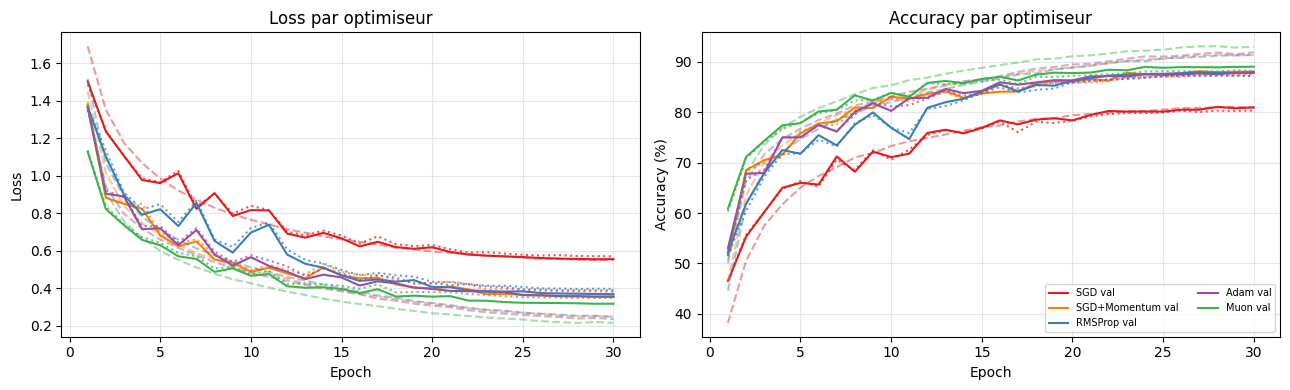
\includegraphics[width=\textwidth]{images/lr-epochs.png}
    \caption{Évolution du taux d'apprentissage par époque}
  \end{figure}

  \begin{table}[H]
    \centering
    \caption{Hyperparamètres des optimiseurs utilisés}
    \label{tab:optimizer-hparams}
    \begin{tabular}{p{3.2cm}p{6.2cm}p{3.2cm}}
      \toprule
      \textbf{Optimiseur} & \textbf{Paramètres principaux} & \textbf{LR initial} \\
      \midrule
      SGD & Aucun momentum & $10^{-2}$ \\
      SGD avec momentum & $\mu = 0.9$ & $10^{-2}$ \\
      Muon & Orthogonalisation Newton-Schulz & $10^{-2}$ \\
      RMSProp & $\rho = 0.9$, $\epsilon = 10^{-8}$ & $1.39 \times 10^{-3}$ \\
      Adam & $\beta_1 = 0.9$, $\beta_2 = 0.999$, $\epsilon = 10^{-8}$ & $1.39 \times 10^{-3}$ \\
      \bottomrule
    \end{tabular}
  \end{table}

% \vspace{0.3}

% \begin{table}[H]
%   \centering
%   \caption{Résultat le meilleur taux d’apprentissage}
%   \label{tab:optim}
%   \begin{tabular}{lll}
%     \toprule
%     \textbf{Optimiseur} & \textbf{Paramètres} & \textbf{Taux d'apprentissage} \\
%     \midrule
% SGD              & -                               & $10^{-2}$ \\
% SGD + Momentum   & $\mu = 0.9$                     & $10^{-2}$ \\
% Muon          & $\epsilon = 10^{-8}$            & $10^{-2}$ \\
% RMSProp          & $\rho = 0.9$, $\epsilon = 10^{-8}$ & $1.39 \times 10^{-3}$ \\
% Adam             & $\beta_1=0.9$, $\beta_2=0.999$  & $1.39 \times 10^{-3}$ \\
%     \bottomrule
%   \end{tabular}
% \end{table}

\subsection{Métriques et reproductibilité}

Pour comparer les optimiseurs de manière cohérente, nous utilisons les mêmes
  métriques pour chaque expérience. La performance est évaluée principalement
  par
  l'accuracy sur les ensembles d'entraînement, de validation et de test. Nous
  suivons
  également la précision macro, qui mesure la qualité des prédictions en tenant
  compte
  des dix classes de CIFAR-10 de manière équilibrée.

  En plus des métriques de classification, nous analysons la perte
  d'entraînement et
  de test afin d'observer la vitesse de convergence de chaque optimiseur.
  L'écart de
  généralisation est calculé comme la différence entre l'accuracy d'entraînement
  et
  l'accuracy de test :
  \begin{equation}
    \text{Gap}_{\text{gén.}} =
    \text{Accuracy}_{\text{train}} - \text{Accuracy}_{\text{test}}.
  \end{equation}
  Un écart élevé indique que le modèle s'adapte davantage aux données
  d'entraînement,
  tandis qu'un écart faible suggère une meilleure capacité de généralisation.

  Afin de rendre les résultats reproductibles, nous fixons la graine aléatoire à $42$ pour PyTorch et NumPy. Tous les optimiseurs sont entraînés avec la même architecture, le même découpage des données, le même nombre d'époques $30$), la même taille de batch ($128$) et le même scheduler de taux d'apprentissage. Les différences observées proviennent donc principalement du choix de l'optimiseur.

% ==========================================================
\section{Résultats et analyse}
\label{sec:resultats}
% ==========================================================

\subsection{Courbes de convergence}
\begin{figure}[H]
  \centering
  \begin{subfigure}{\textwidth}
    \centering
    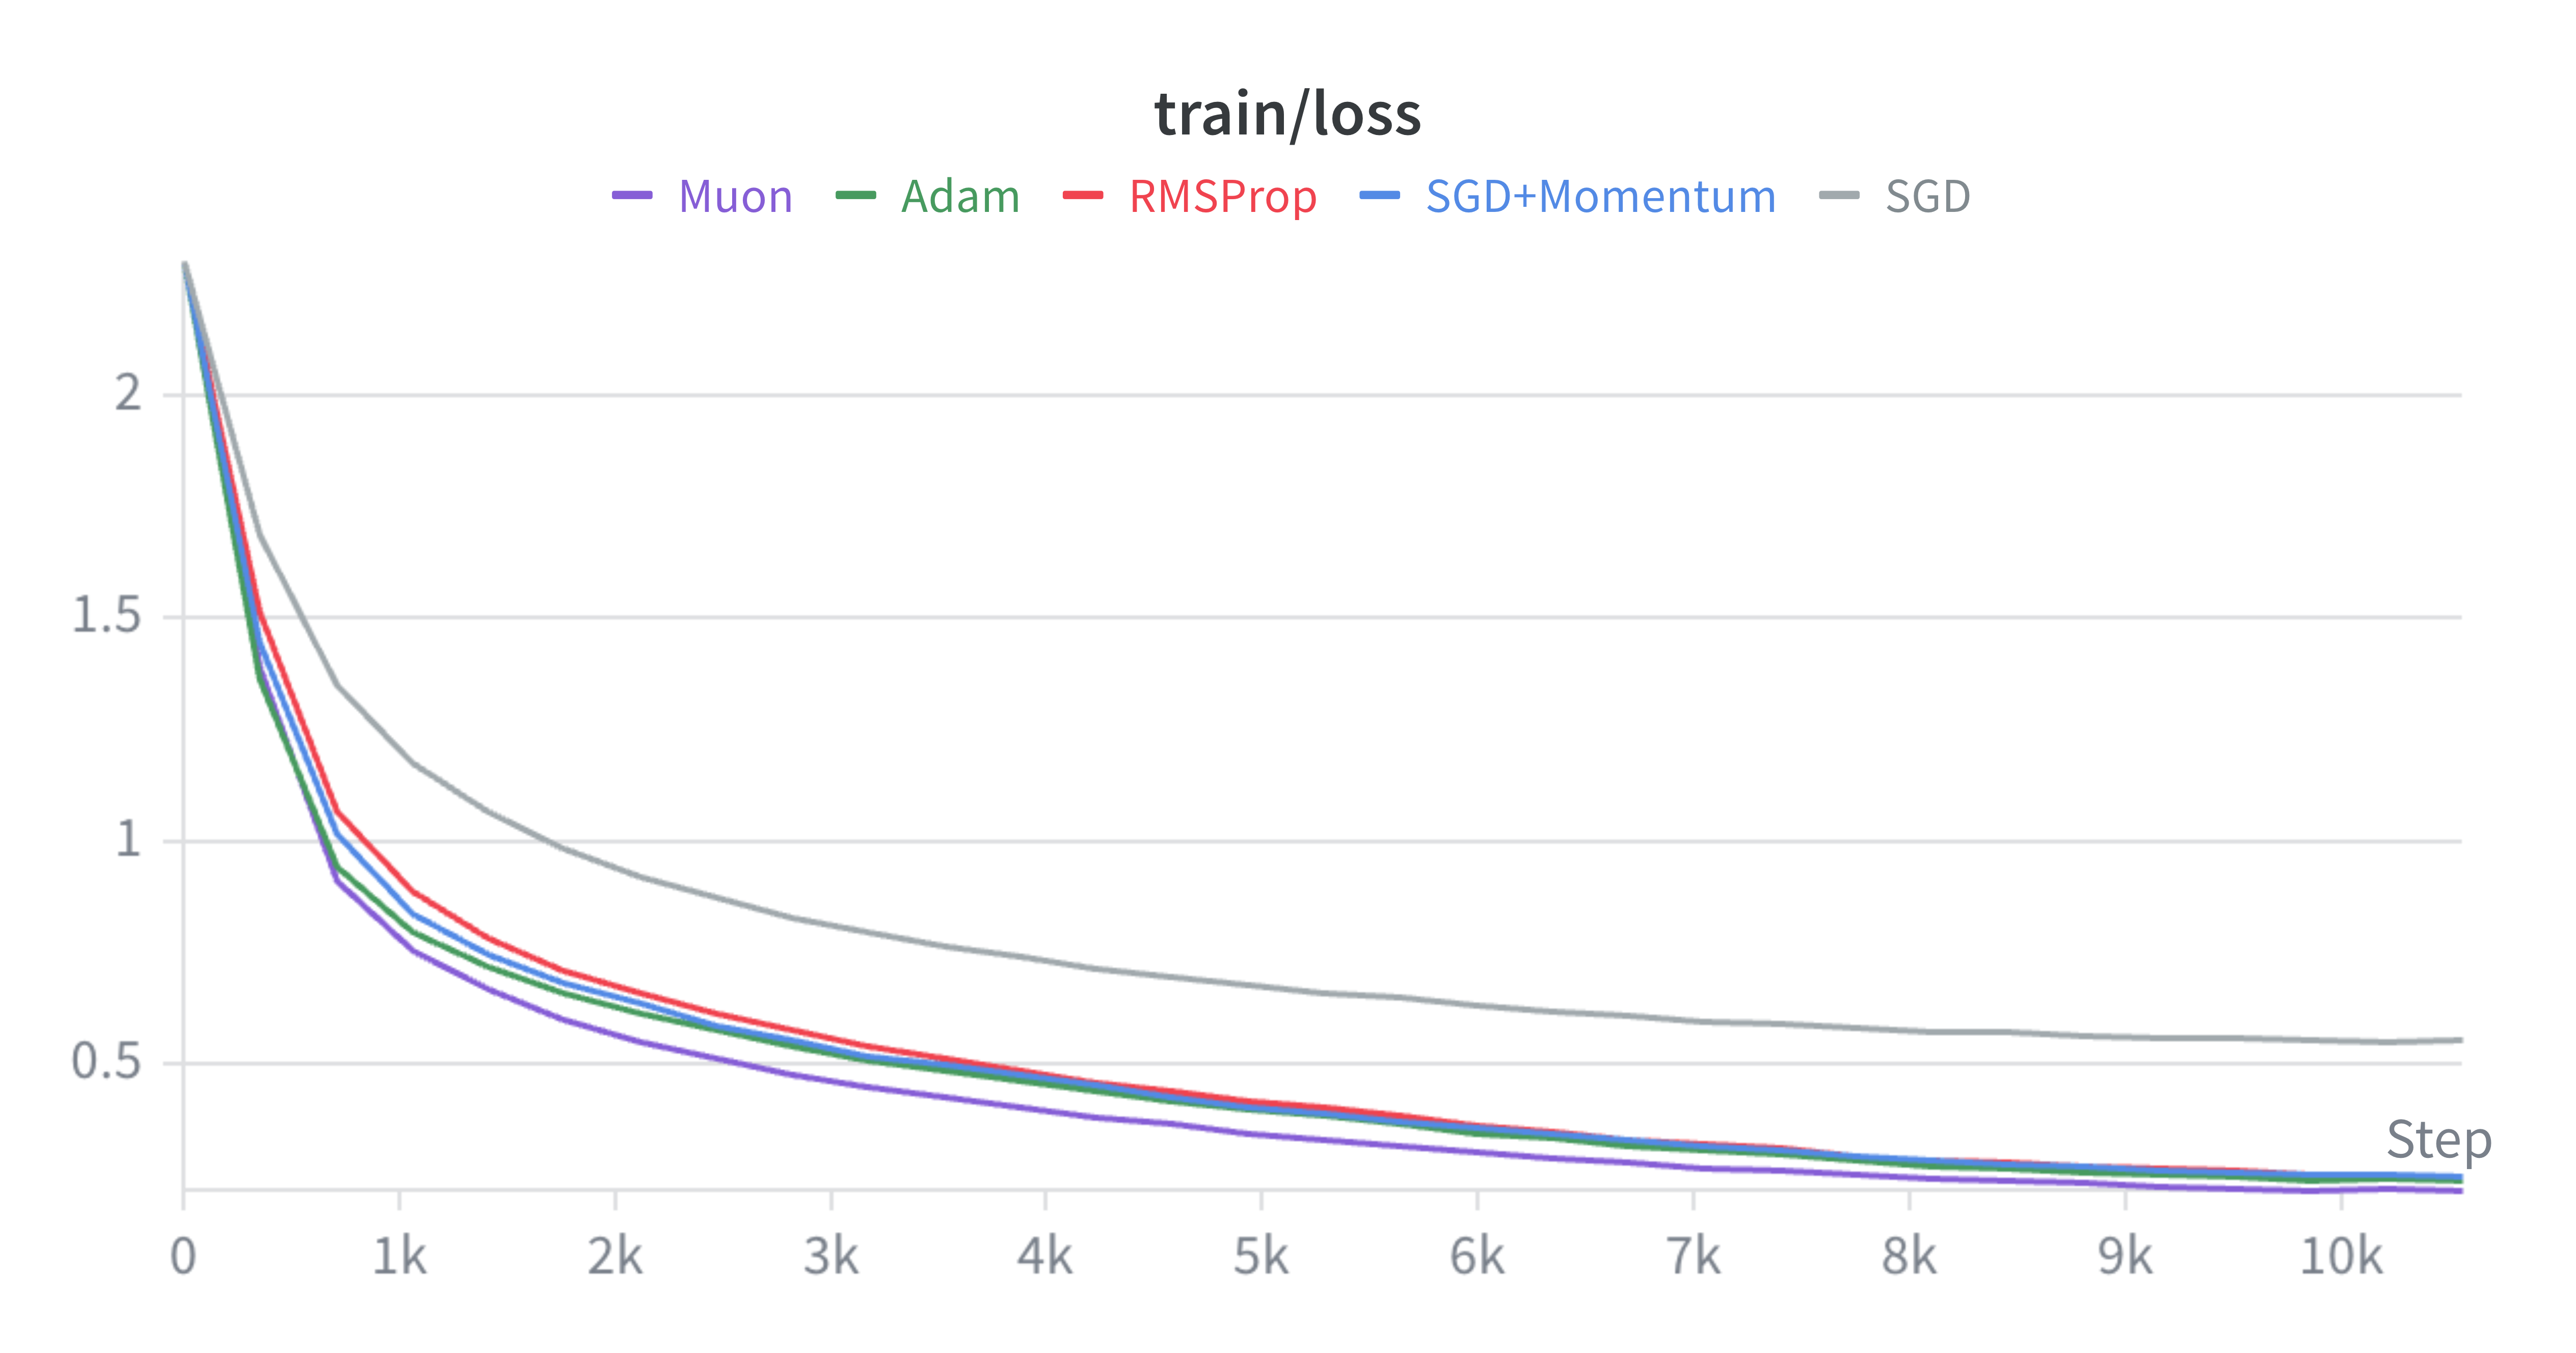
\includegraphics[width=\textwidth]{images/train-loss.png}
    \caption{Courbes de loss sur l'entraînement}
  \end{subfigure}

  \vspace{0.5cm}

  \begin{subfigure}{0.48\textwidth}
    \centering
    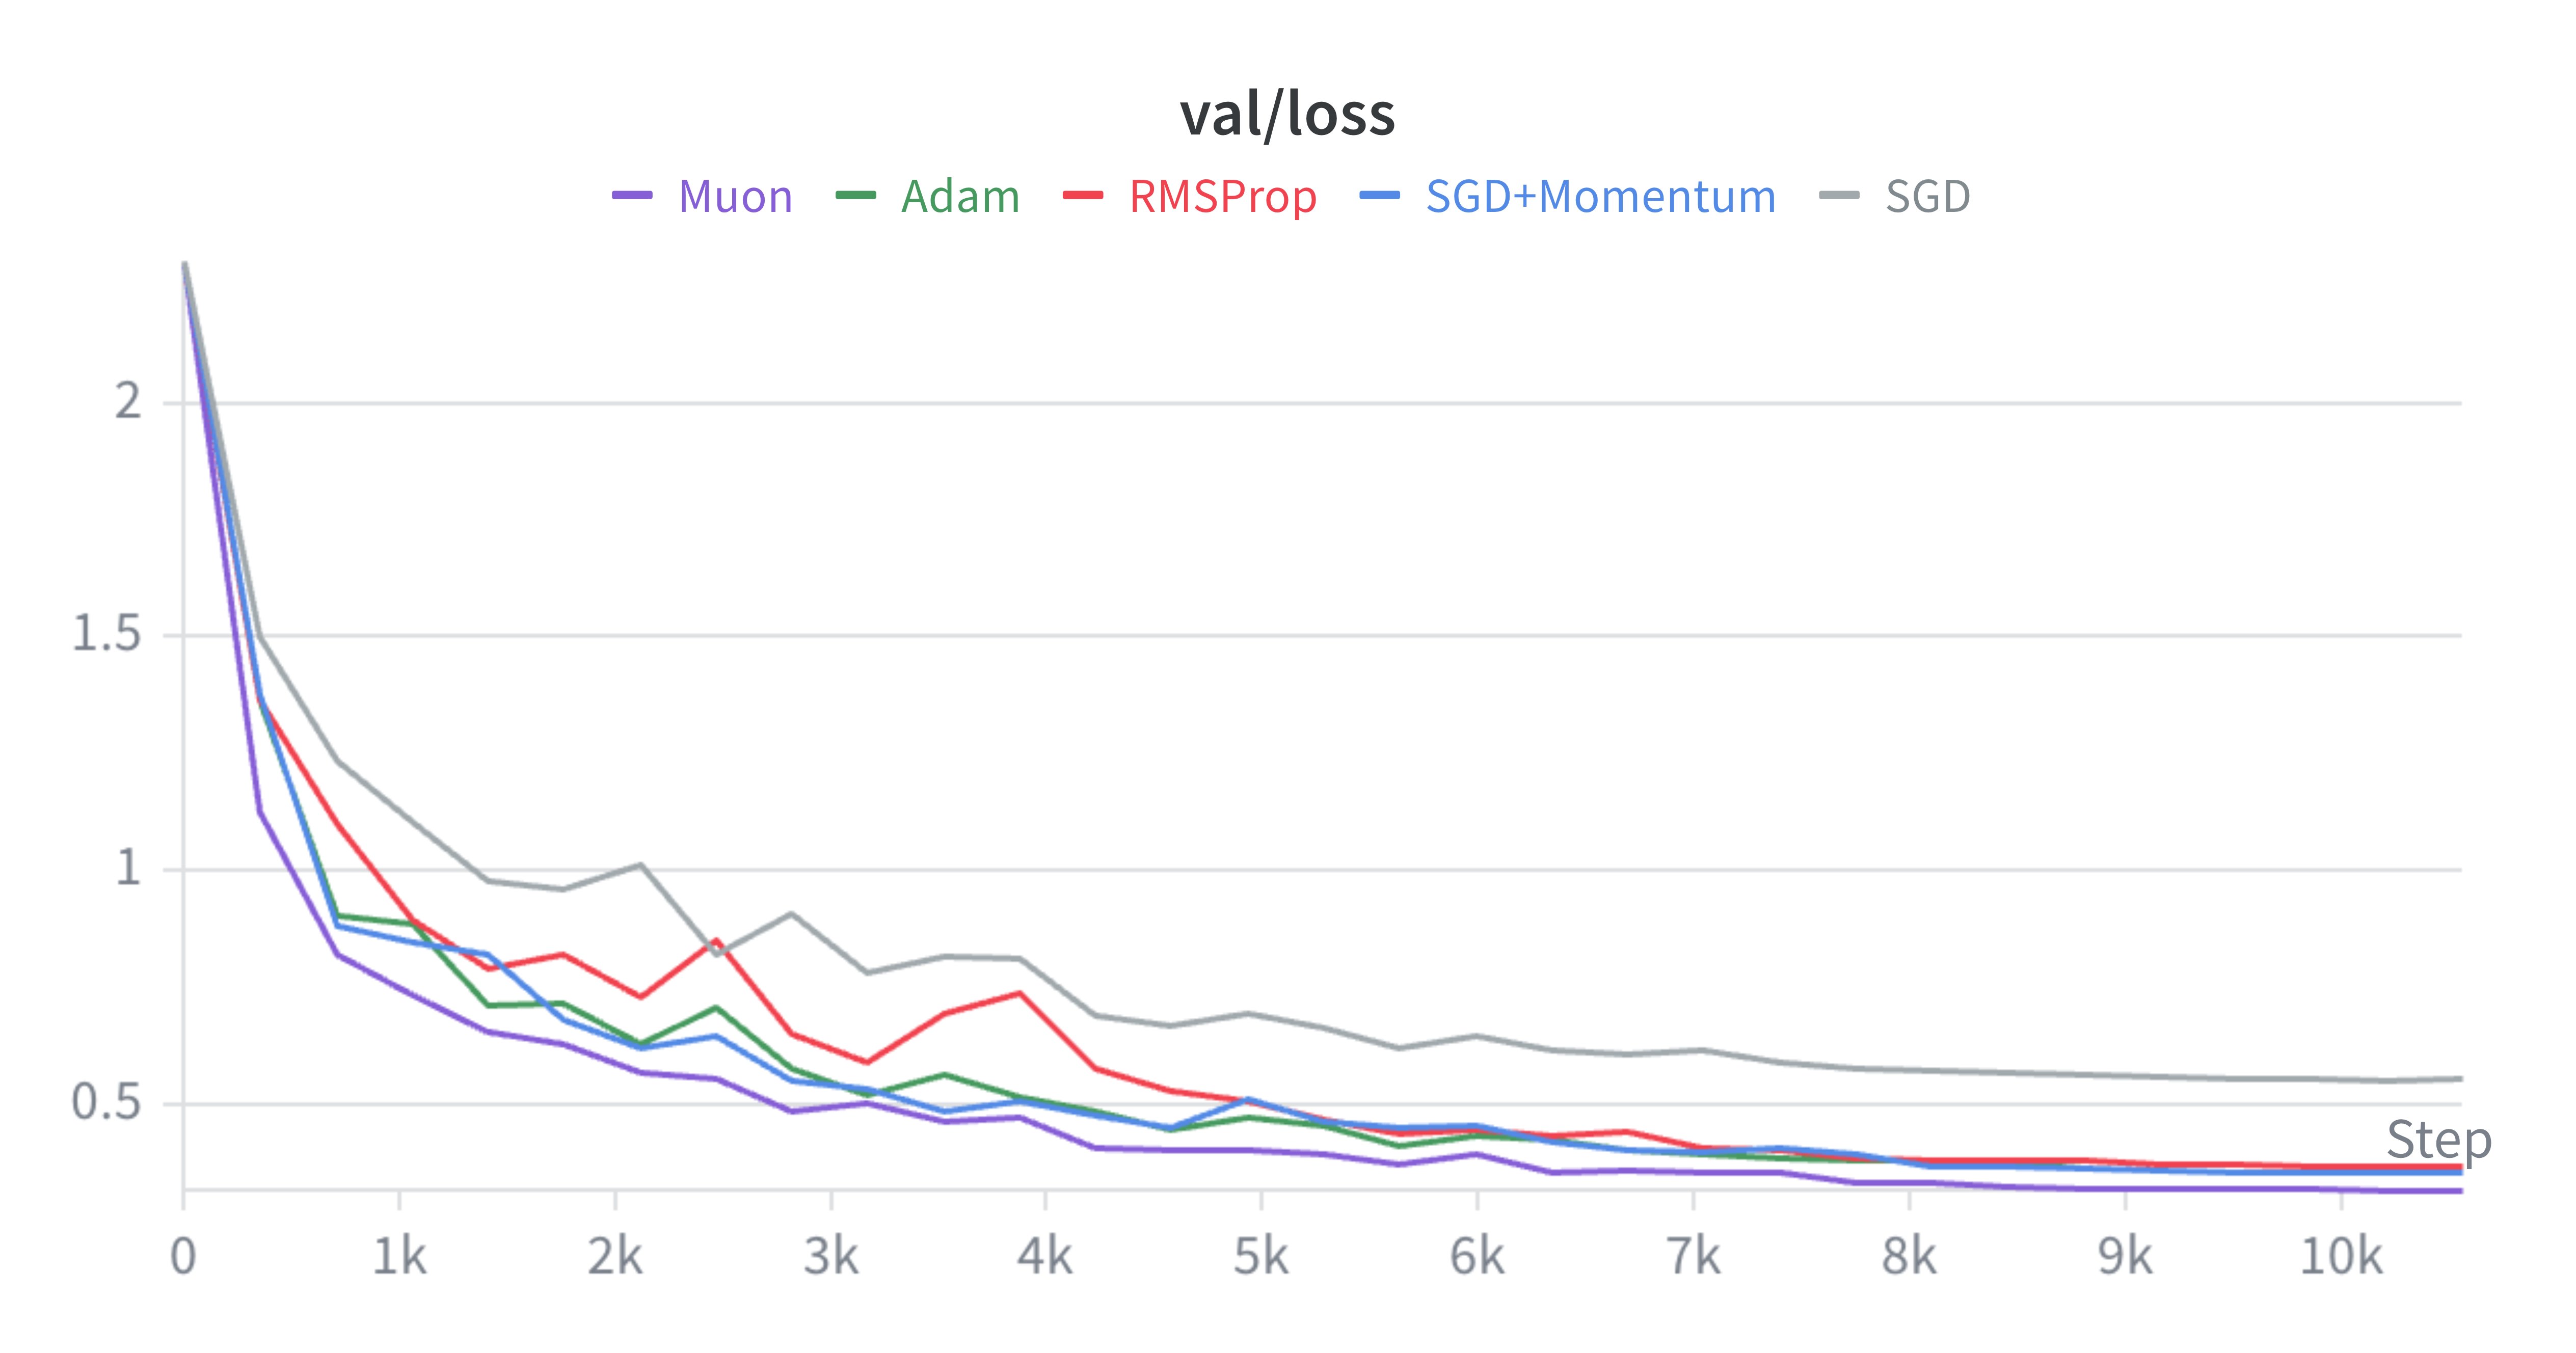
\includegraphics[width=\textwidth]{images/val-loss.png}
    \caption{Perte de validation}
  \end{subfigure}
  \hfill
  \begin{subfigure}{0.48\textwidth}
    \centering
    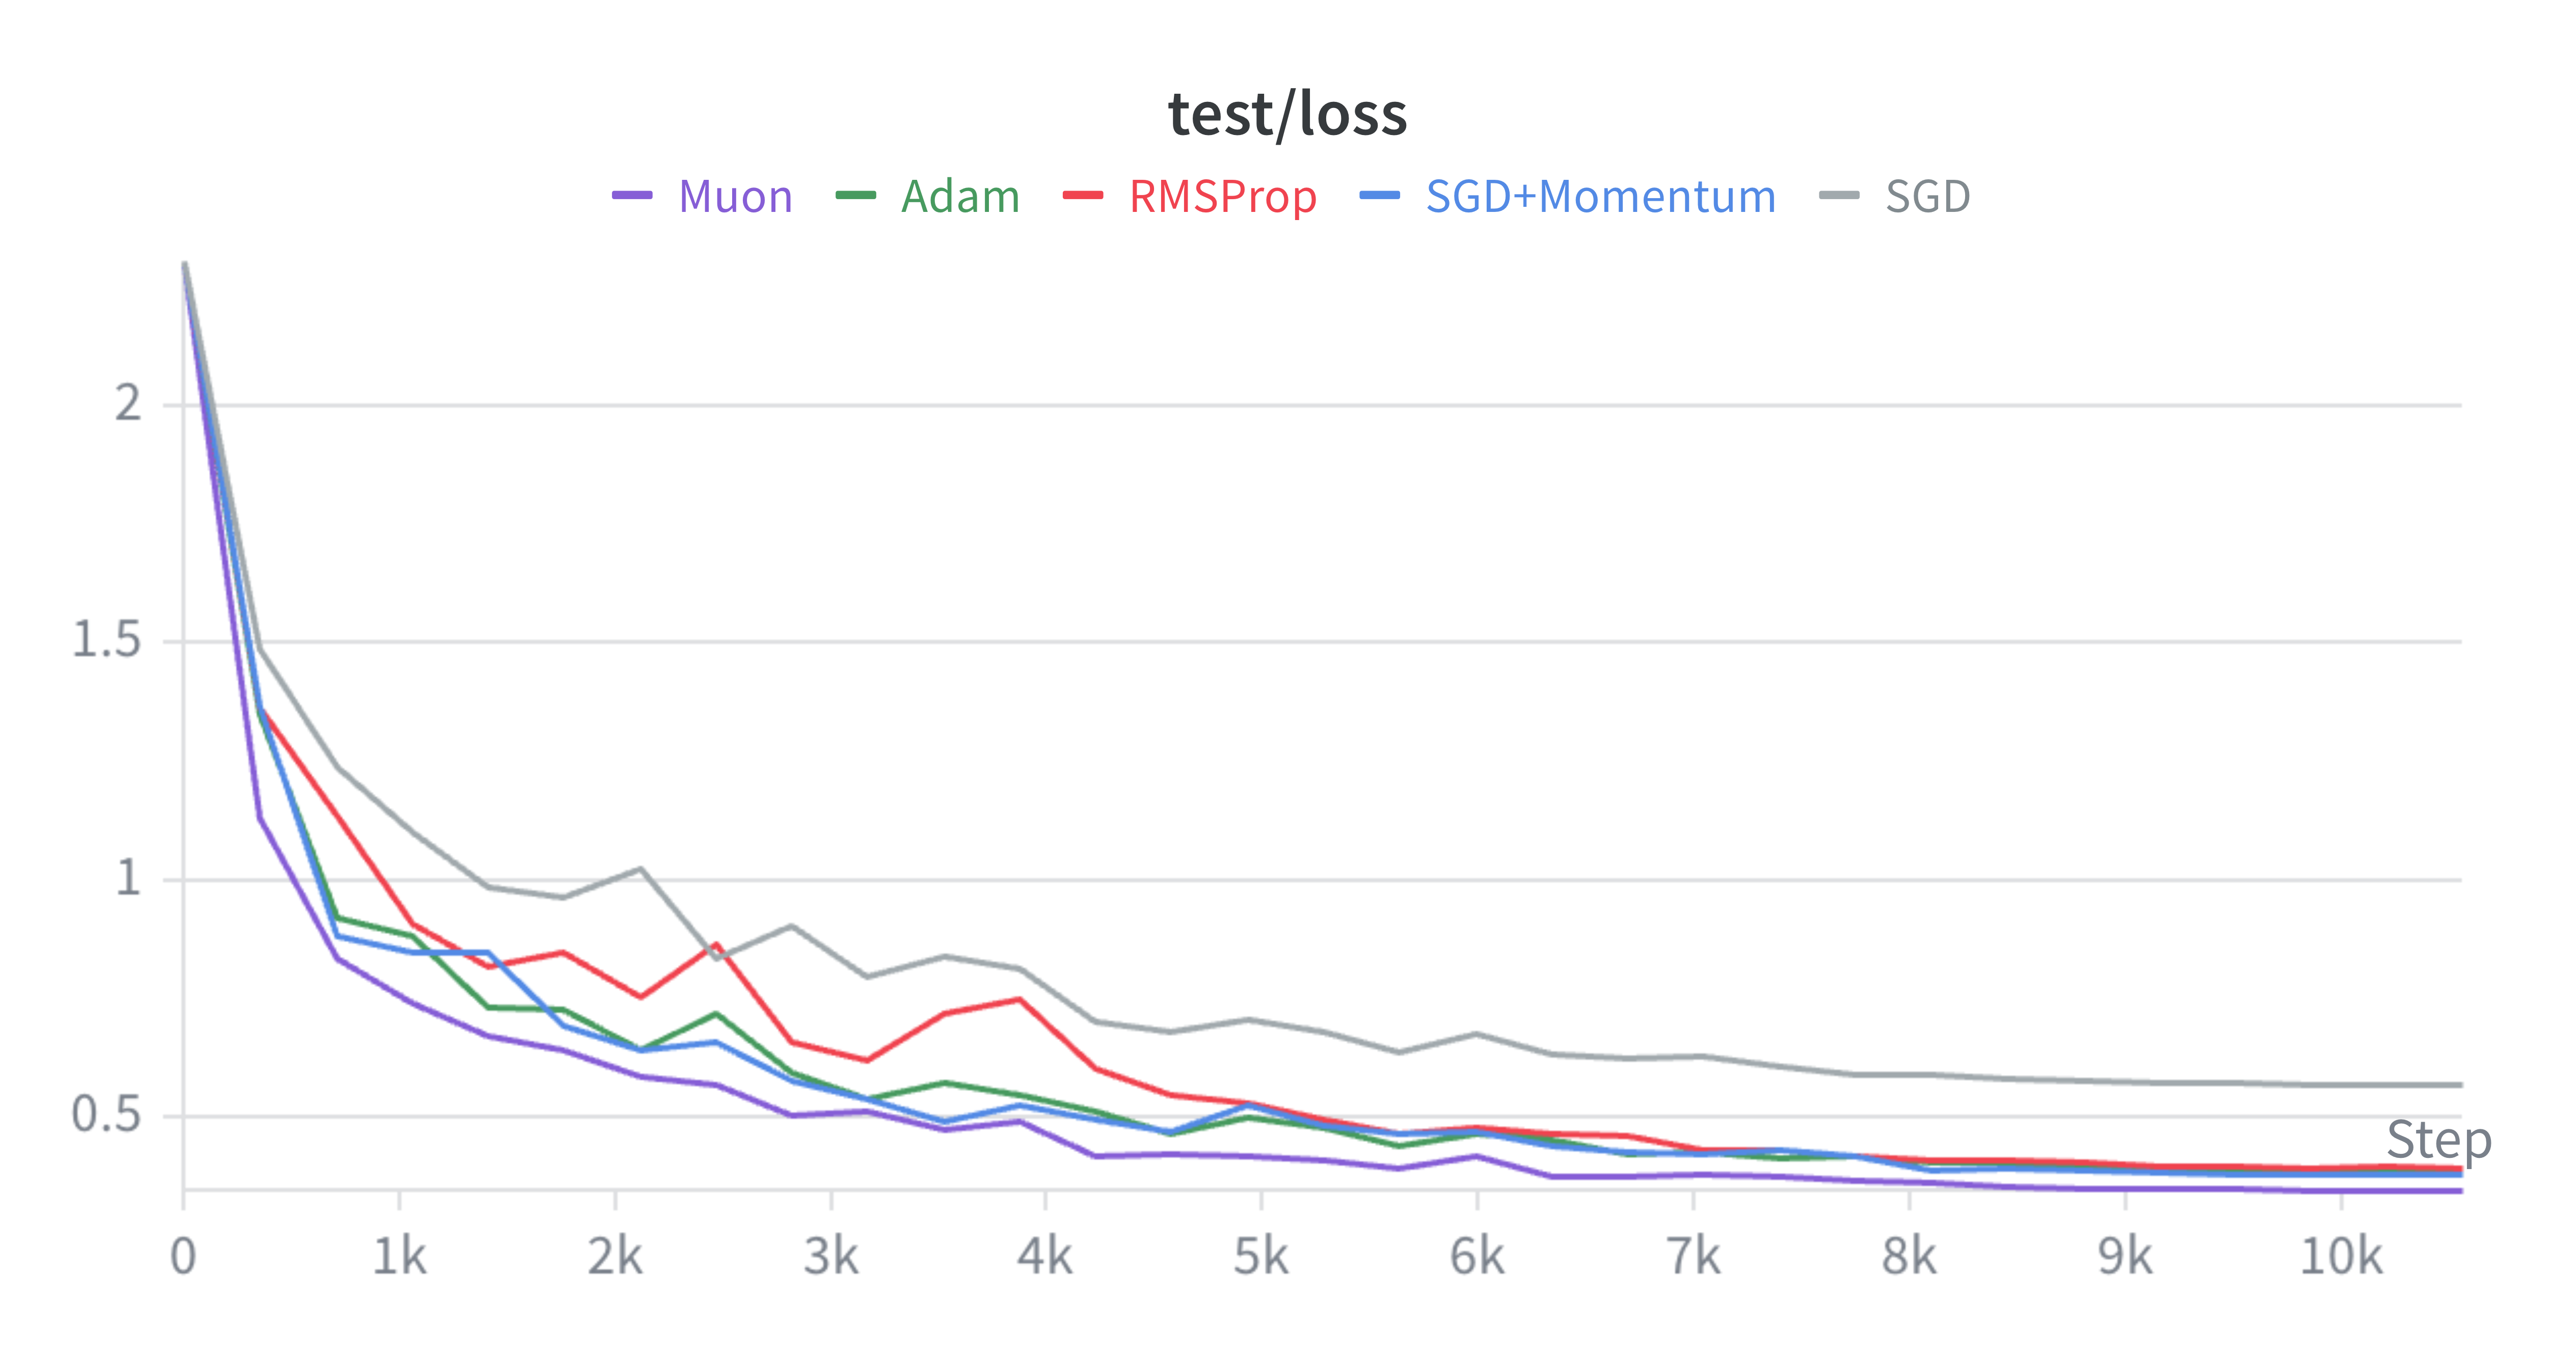
\includegraphics[width=\textwidth]{images/test-loss.png}
    \caption{Perte de test}
  \end{subfigure}

  \caption{Courbes de perte pour les cinq optimiseurs (30 époques)}
  \label{fig:loss-curves}
\end{figure}

 La figure~\ref{fig:loss-curves} montre que tous les optimiseurs réduisent rapidement la perte au début de l'entraînement, puis convergent plus lentement après les premières époques. La différence principale concerne la vitesse de descente et le niveau final atteint. Muon obtient la diminution de perte la plus rapide et termine avec la perte la plus faible sur les ensembles d'entraînement, de validation et de test. 
 
 Adam, RMSProp et SGD avec momentum ont des comportements proches. Ces trois
 méthodes convergent nettement plus vite que SGD seul et atteignent des pertes
 finales similaires. RMSProp présente cependant davantage d'oscillations au
 début sur la validation et le test, ce qui indique une trajectoire moins
 régulière.

SGD seul est l'optimiseur le plus lent. Sa perte diminue de manière stable, mais elle reste nettement plus élevée que celle des autres méthodes pendant toute l'expérience. Cela montre que, dans ce cadre, l'absence de momentum ou d'adaptation du taux d'apprentissage ralentit fortement la convergence.

\begin{figure}[H]
  \centering
  \begin{subfigure}{\textwidth}
    \centering
    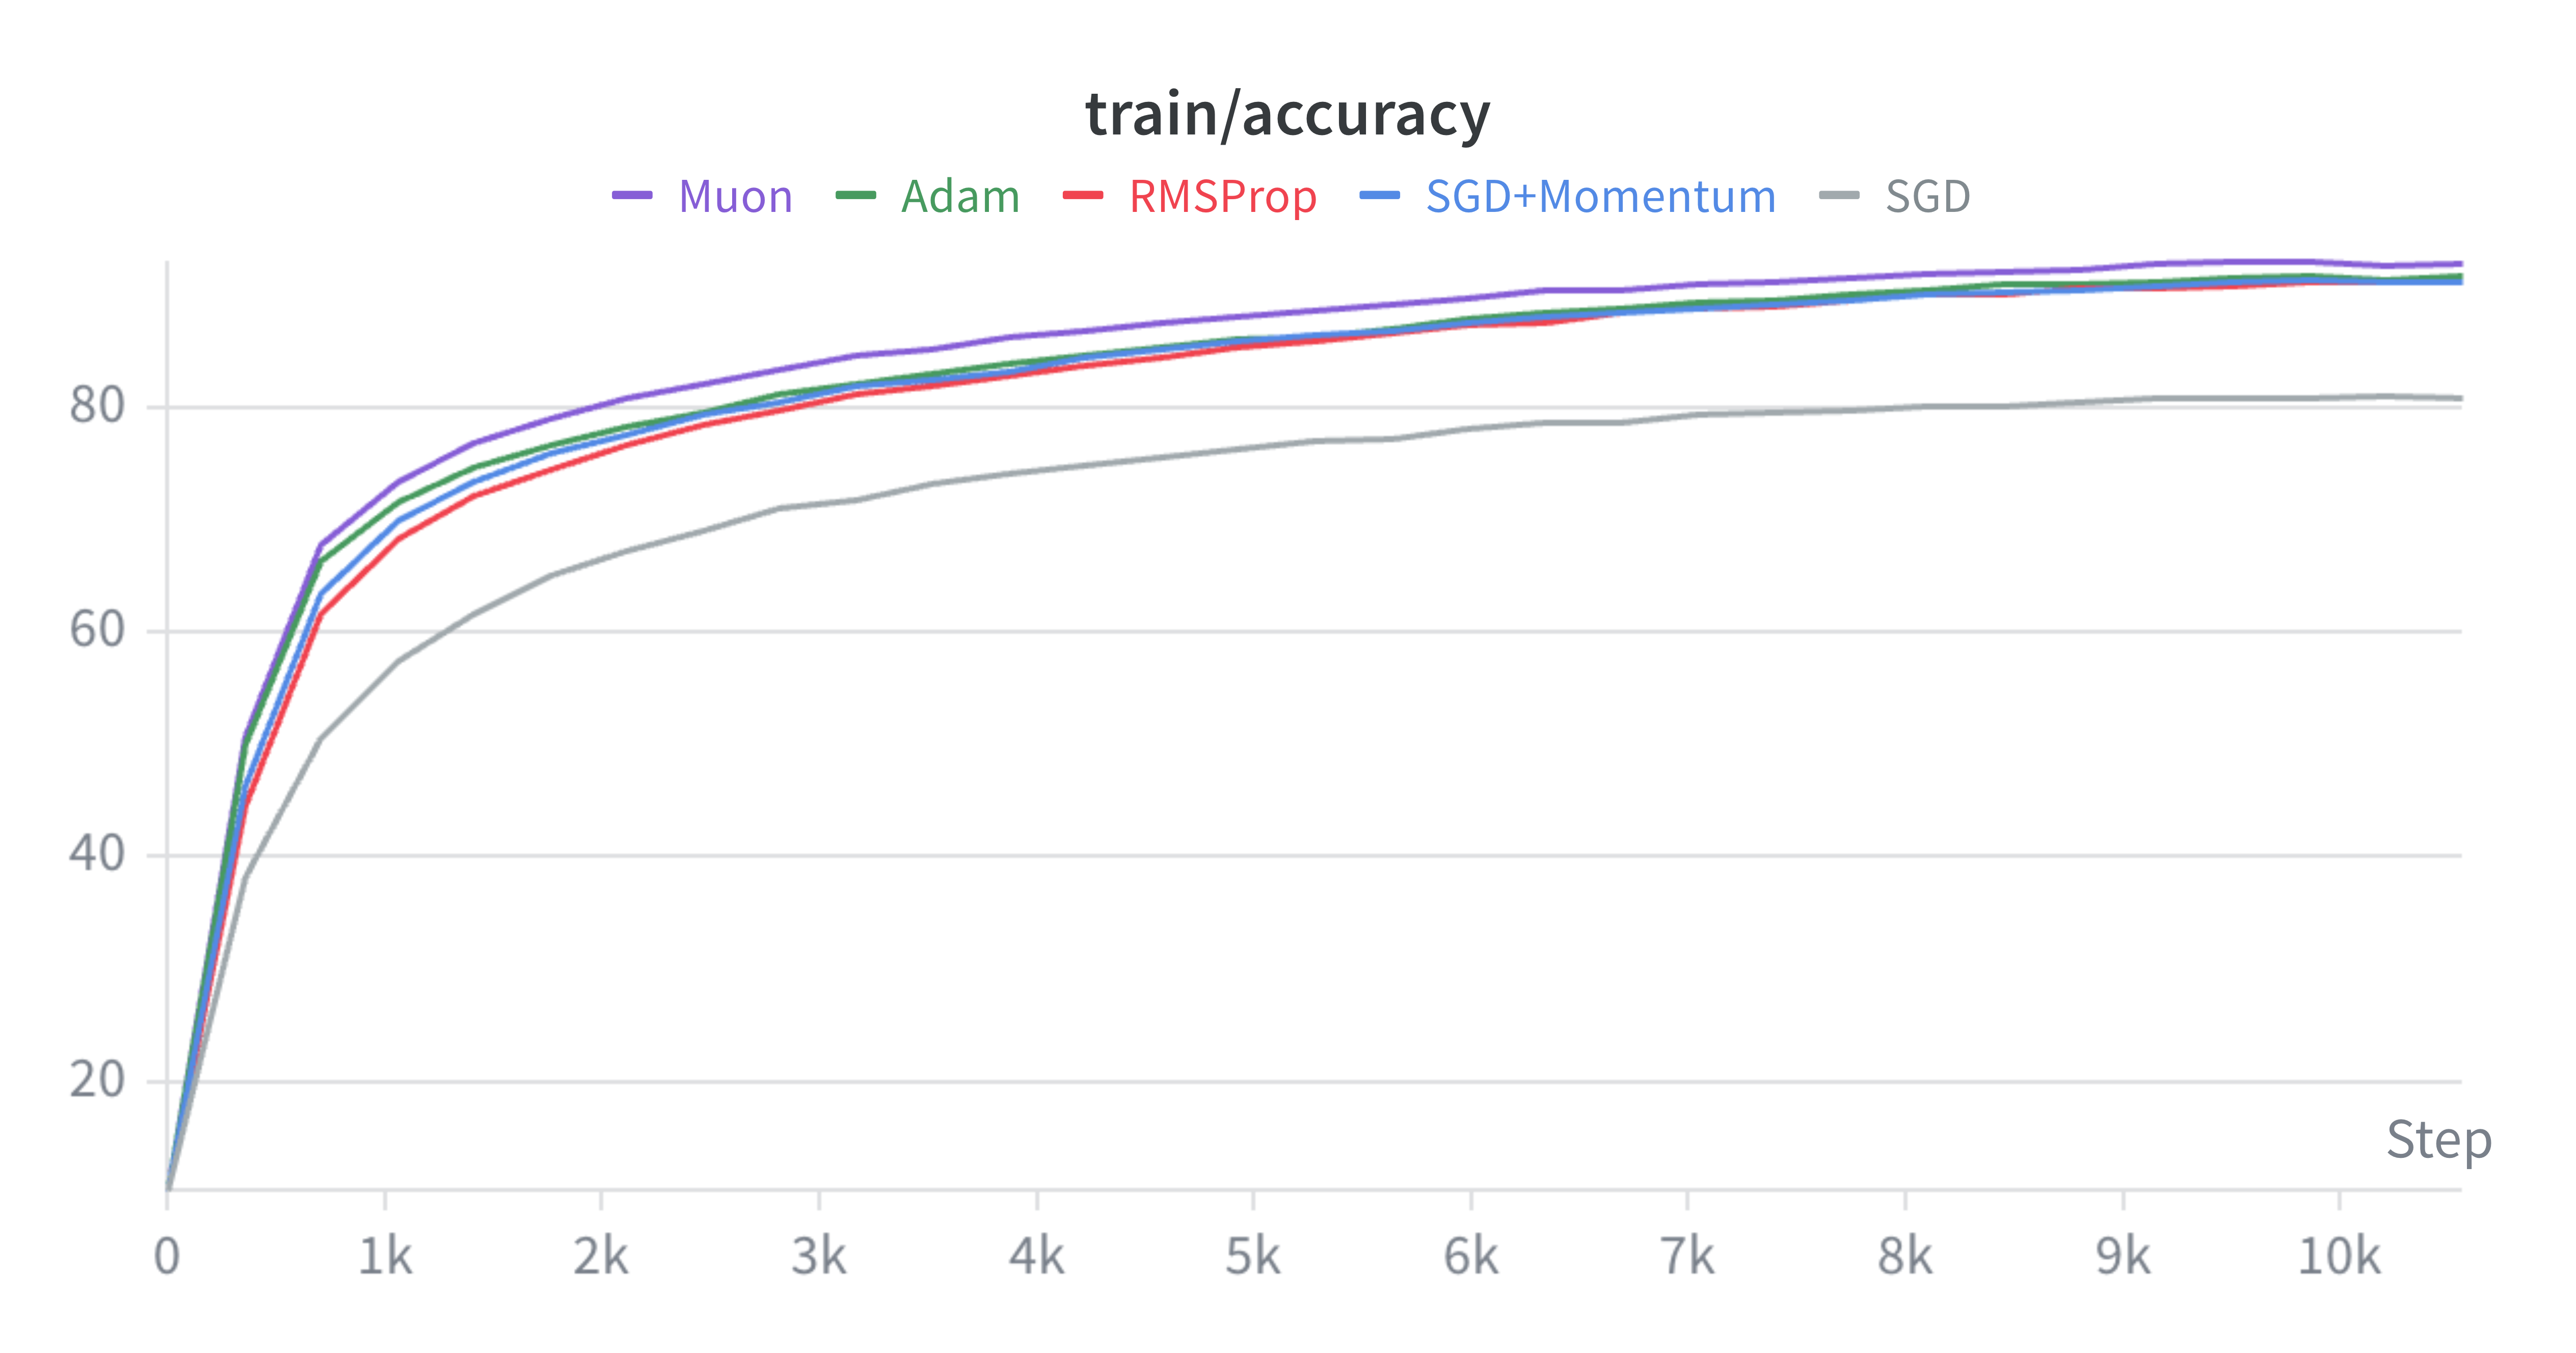
\includegraphics[width=\textwidth]{images/train-acc.png}
    \caption{Accuracy d'entraînement}
  \end{subfigure}

  \vspace{0.5cm}

  \begin{subfigure}{0.48\textwidth}
    \centering
    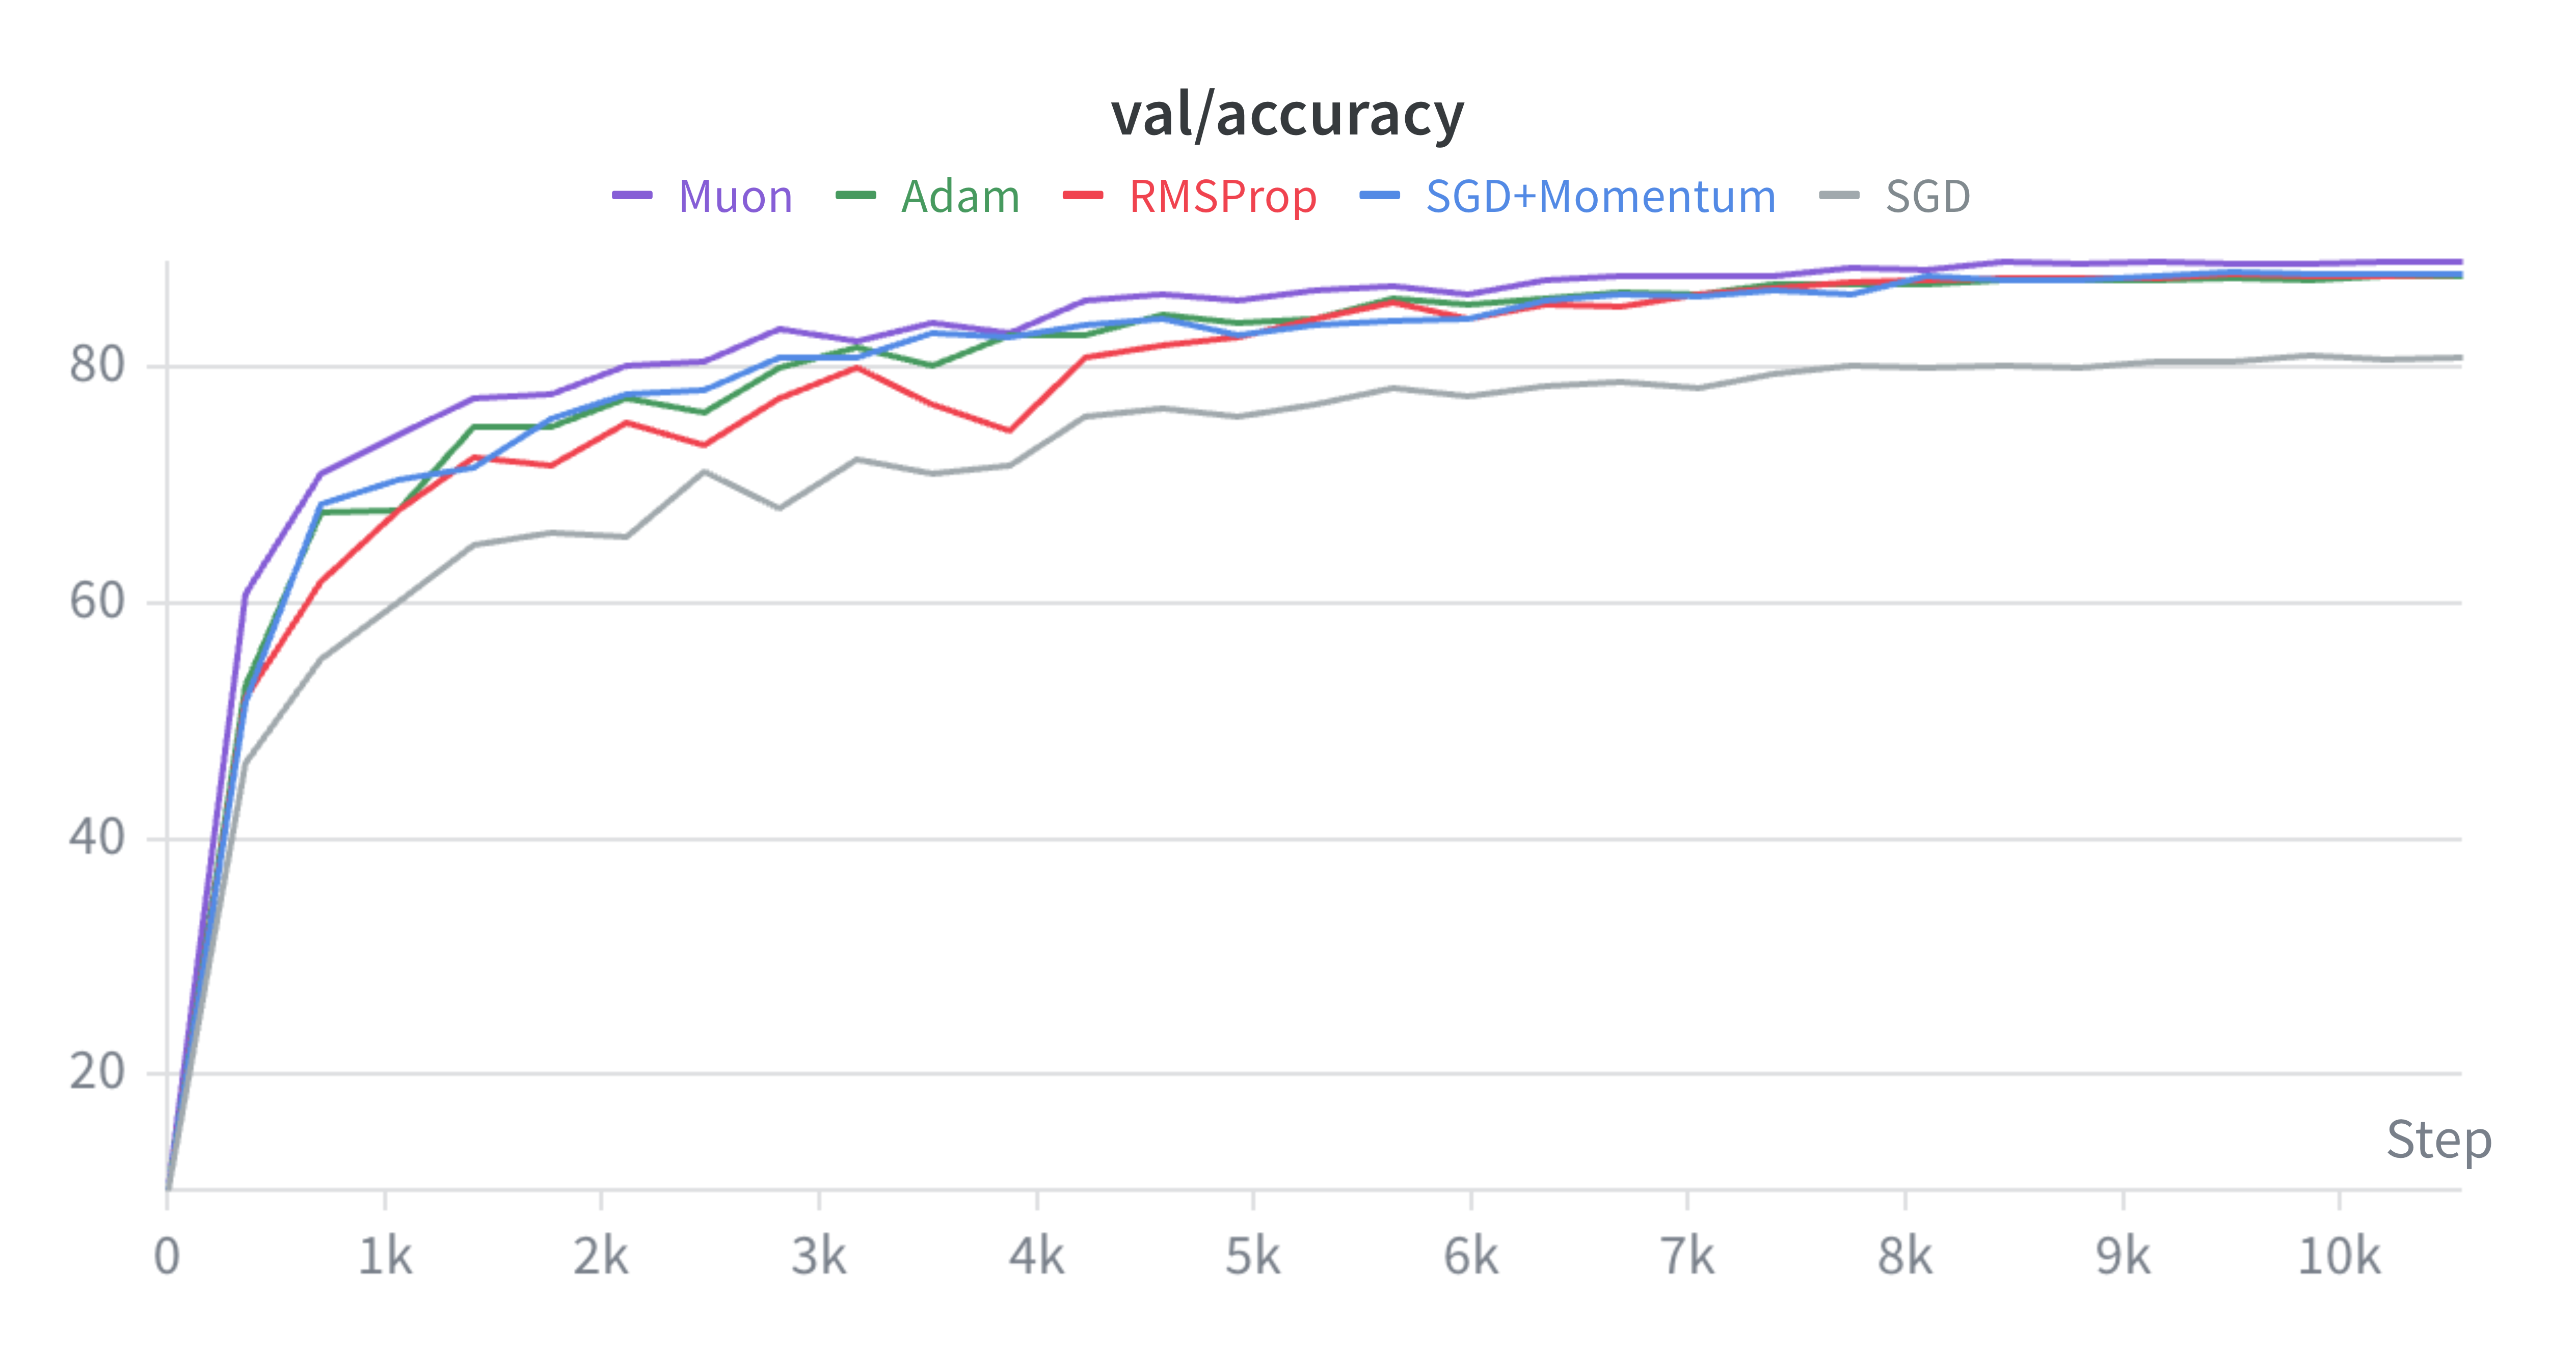
\includegraphics[width=\textwidth]{images/val-acc.png}
    \caption{Accuracy de validation}
  \end{subfigure}
  \hfill
  \begin{subfigure}{0.48\textwidth}
    \centering
    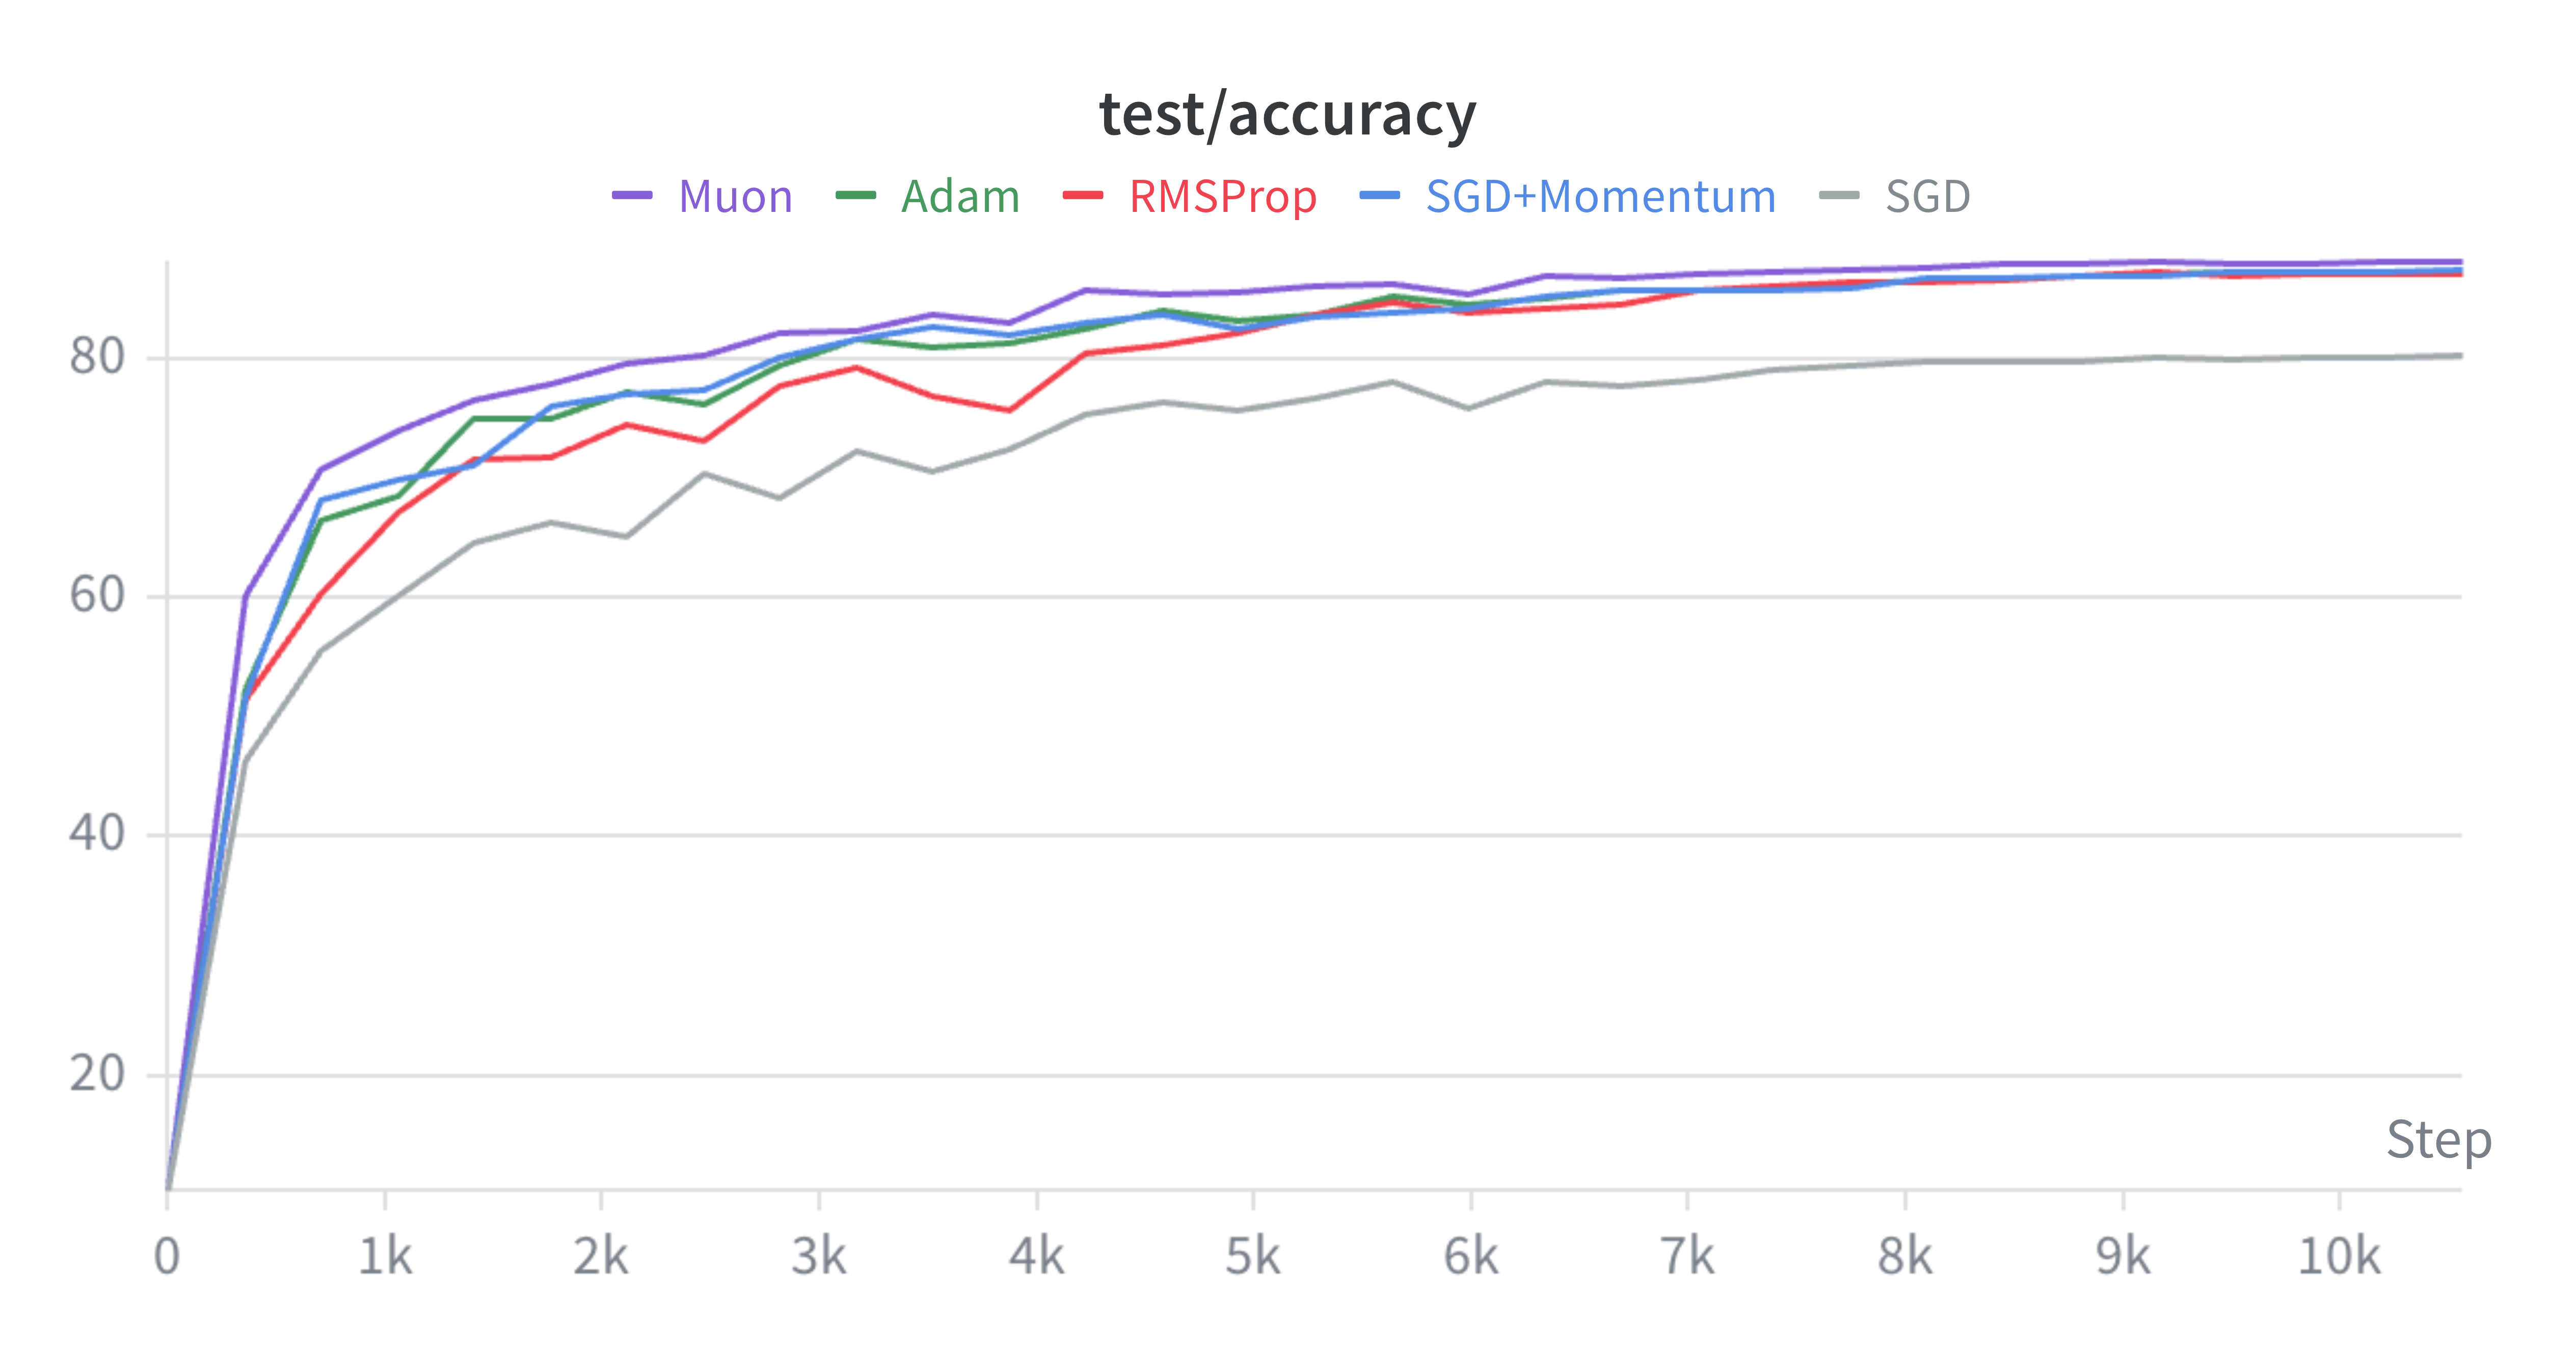
\includegraphics[width=\textwidth]{images/test-acc.png}
    \caption{Accuracy de test}
  \end{subfigure}

  \caption{Courbes d'accuracy pour les cinq optimiseurs (30 époques)}
  \label{fig:acc-curves}
\end{figure}


Muon atteint rapidement une accuracy élevée et conserve un léger avantage
  sur la validation et le test jusqu'à la fin de l'entraînement. Il obtient aussi
  la meilleure accuracy d'entraînement, ce qui indique une optimisation très
  efficace du modèle.

  Adam, RMSProp et SGD+Momentum forment un groupe intermédiaire très proche. Ces
  particulièrement stables après les premières époques, tandis que RMSProp montre
  quelques variations plus visibles au milieu de l'entraînement.

  SGD reste en dessous des autres optimiseurs sur les trois courbes. Il progresse
  régulièrement, mais plus lentement, et son accuracy finale est plus faible. Cela
  confirme que SGD seul nécessite généralement davantage d'époques pour atteindre
  des performances comparables aux méthodes avec momentum, adaptation ou
  orthogonalisation du gradient.

  
\subsection{Précision finale et vitesse de convergence}



\begin{figure}[H]
  \centering
  \begin{subfigure}{\textwidth}
    \centering
    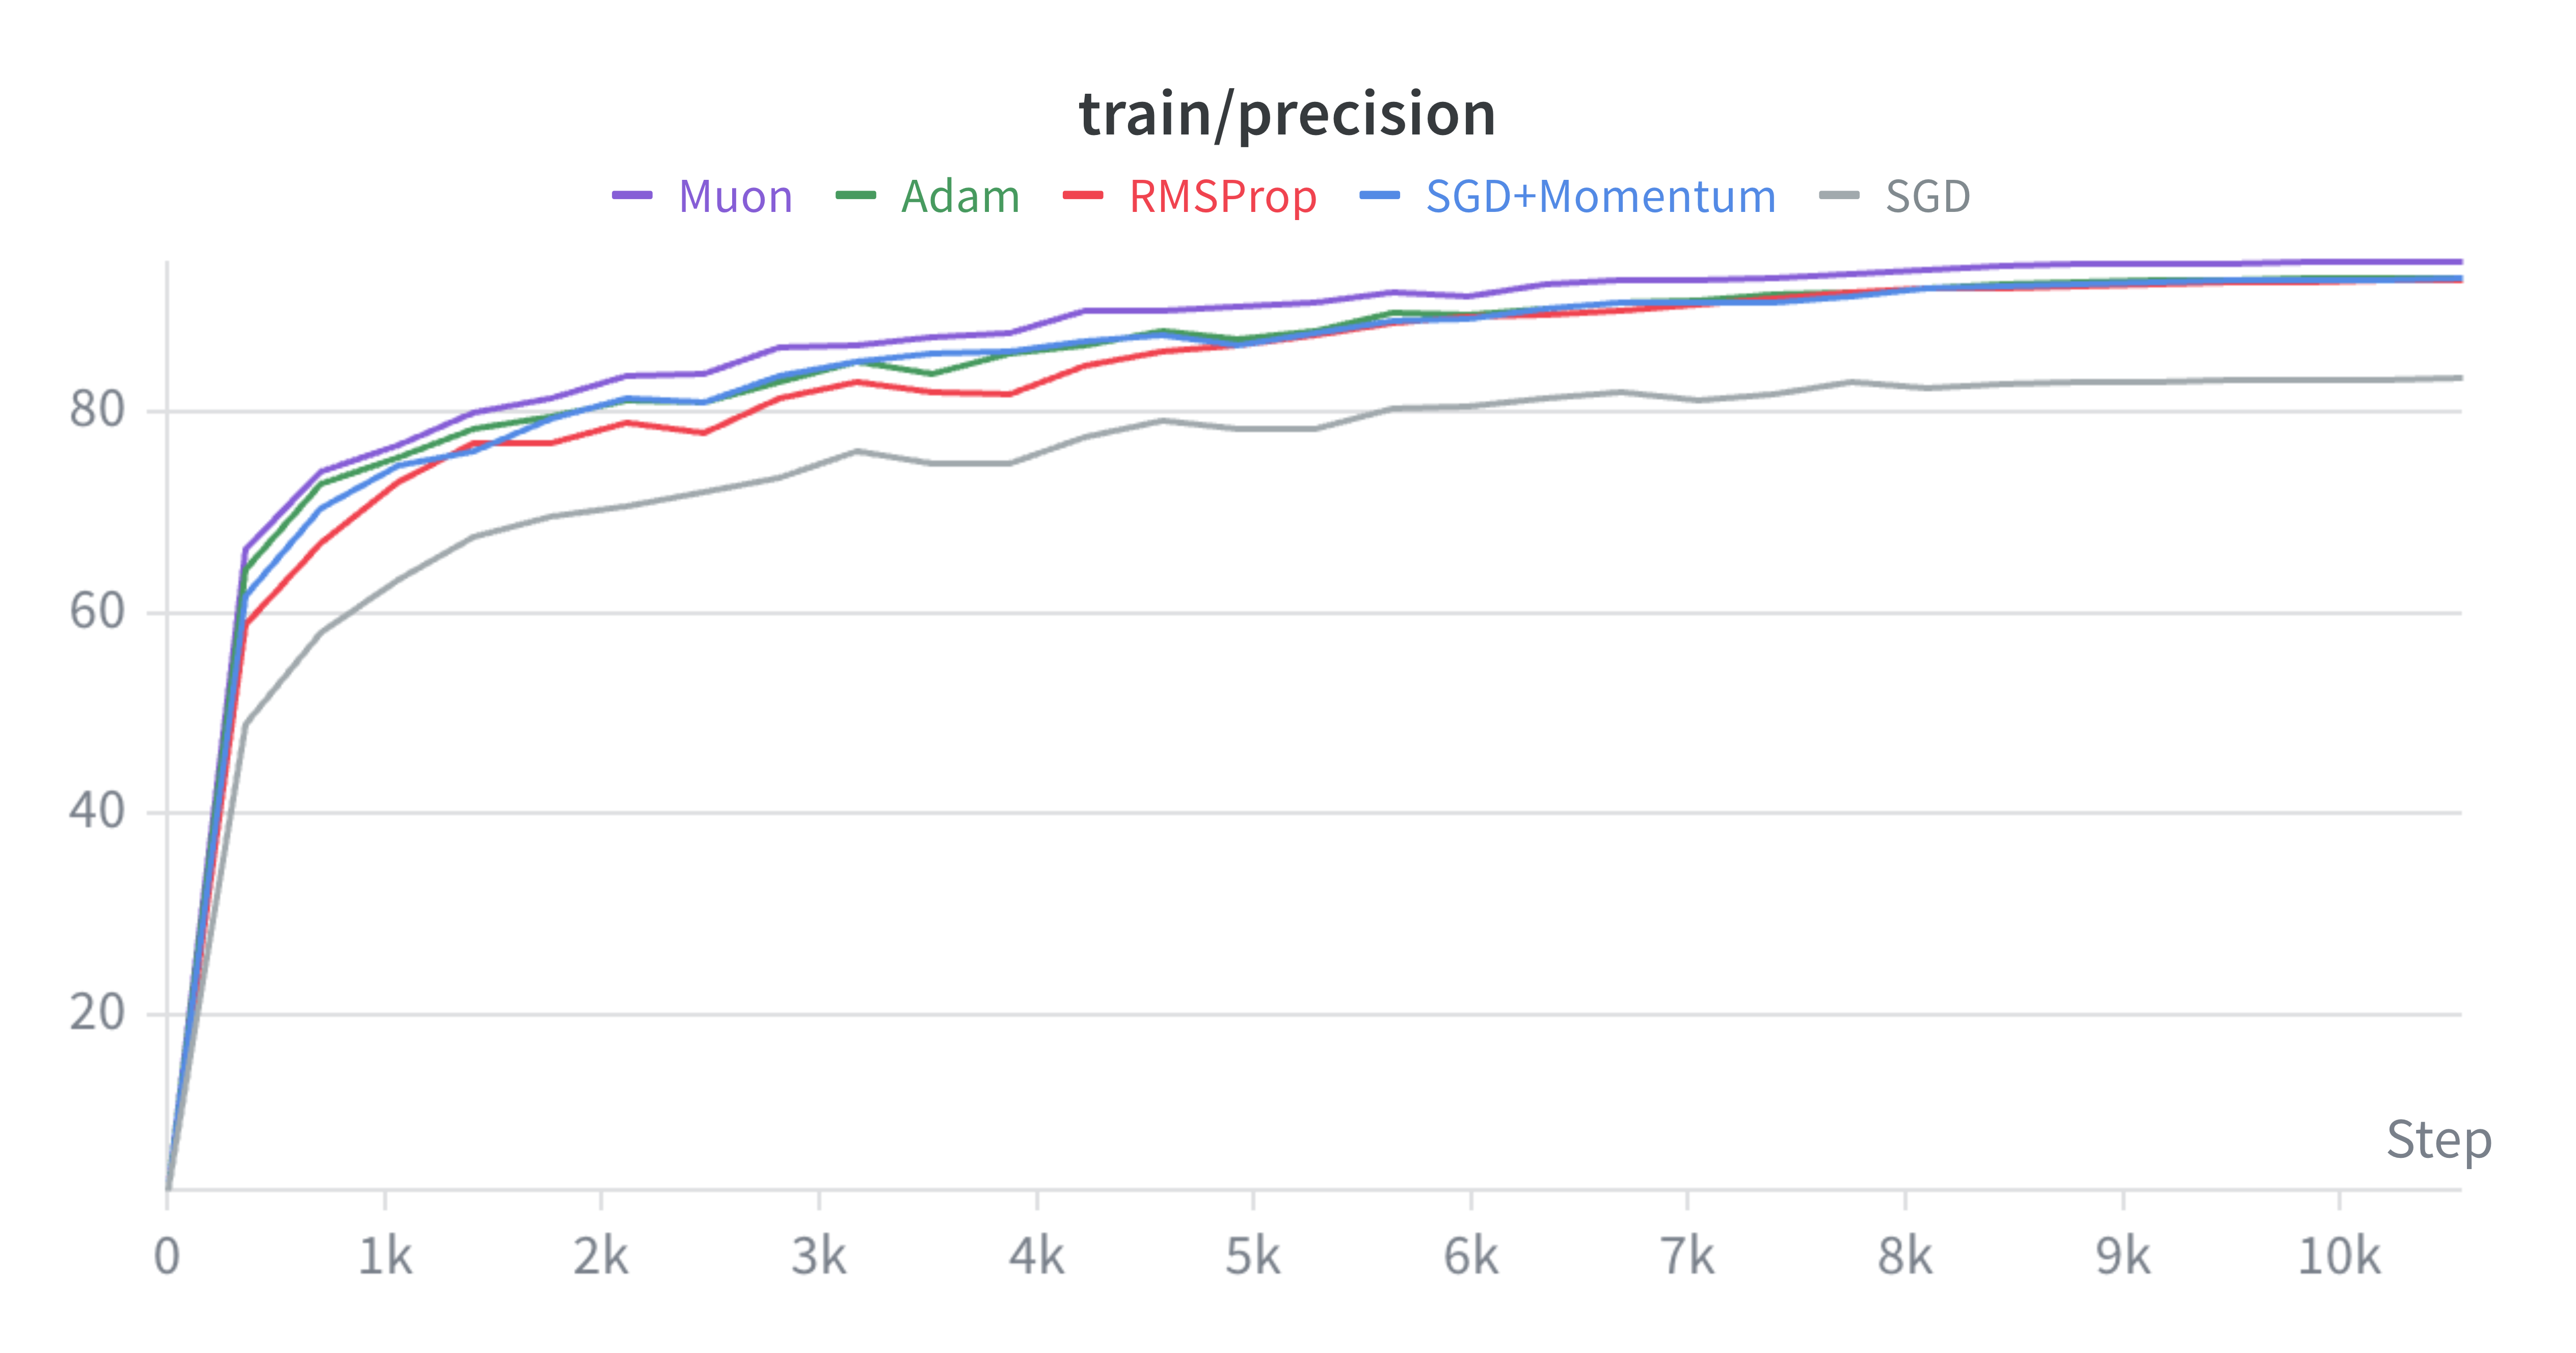
\includegraphics[width=\textwidth]{images/train-precision.png}
    \caption{Precision d'entraînement}
  \end{subfigure}

  \vspace{0.5cm}

  \begin{subfigure}{0.48\textwidth}
    \centering
    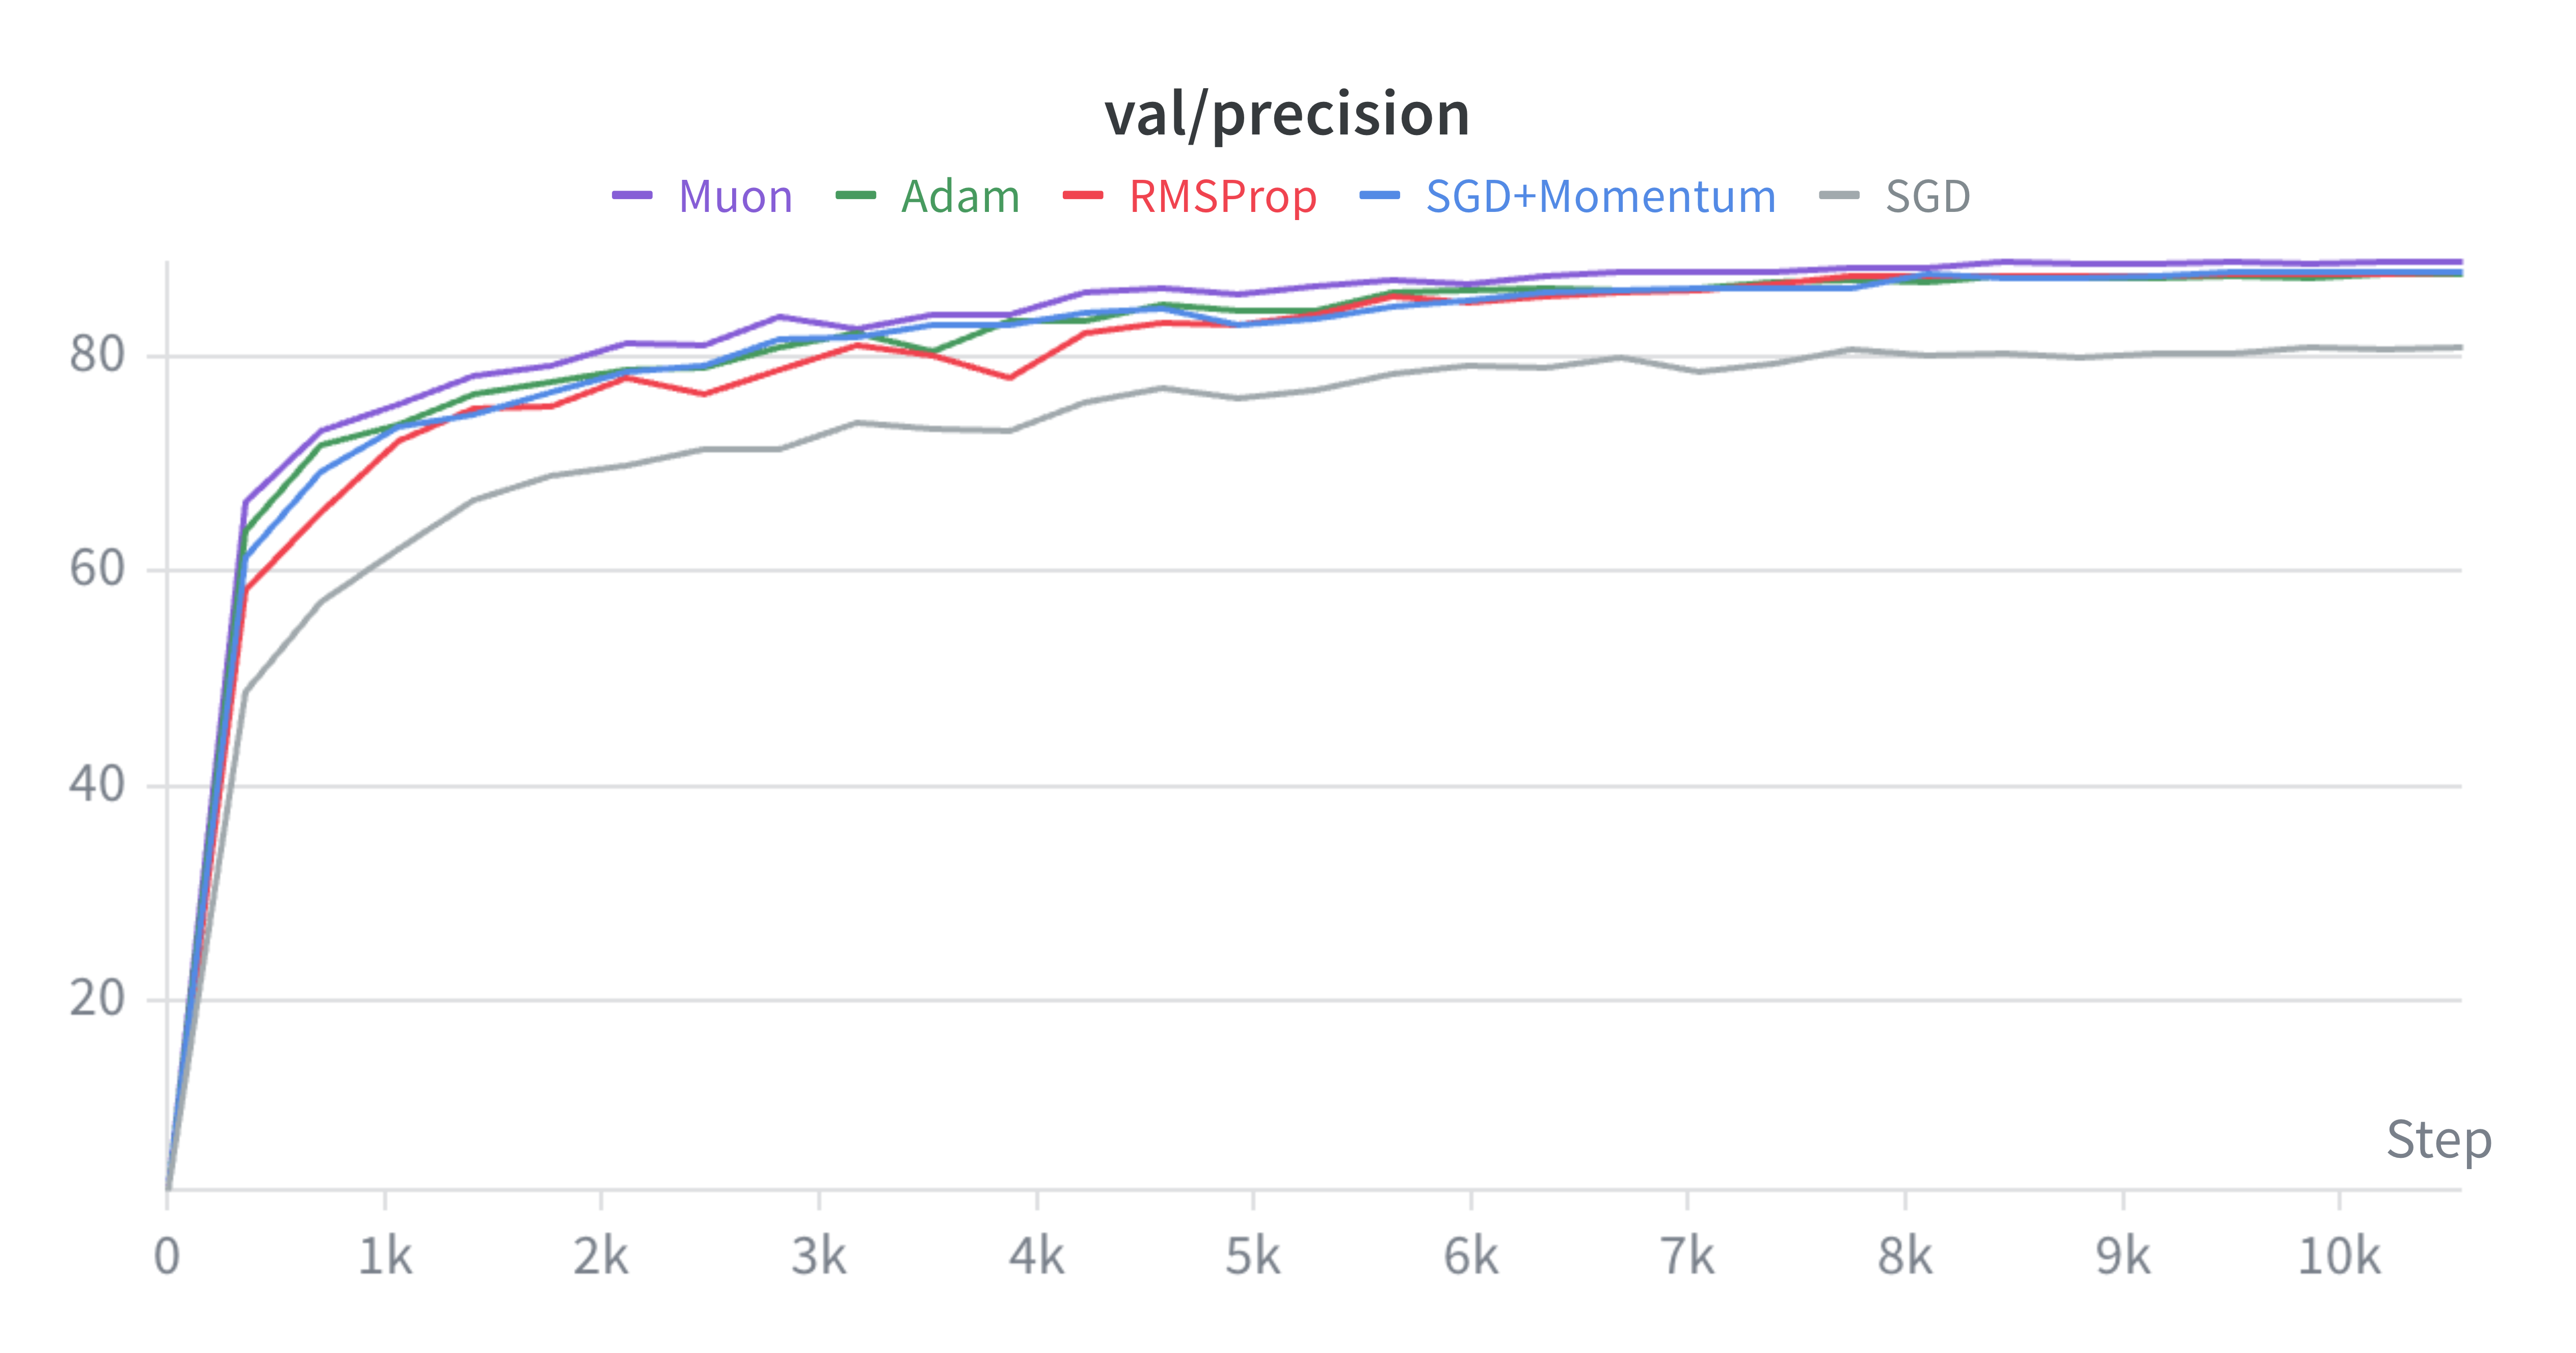
\includegraphics[width=\textwidth]{images/val-precision.png}
    \caption{Precision de validation}
  \end{subfigure}
  \hfill
  \begin{subfigure}{0.48\textwidth}
    \centering
    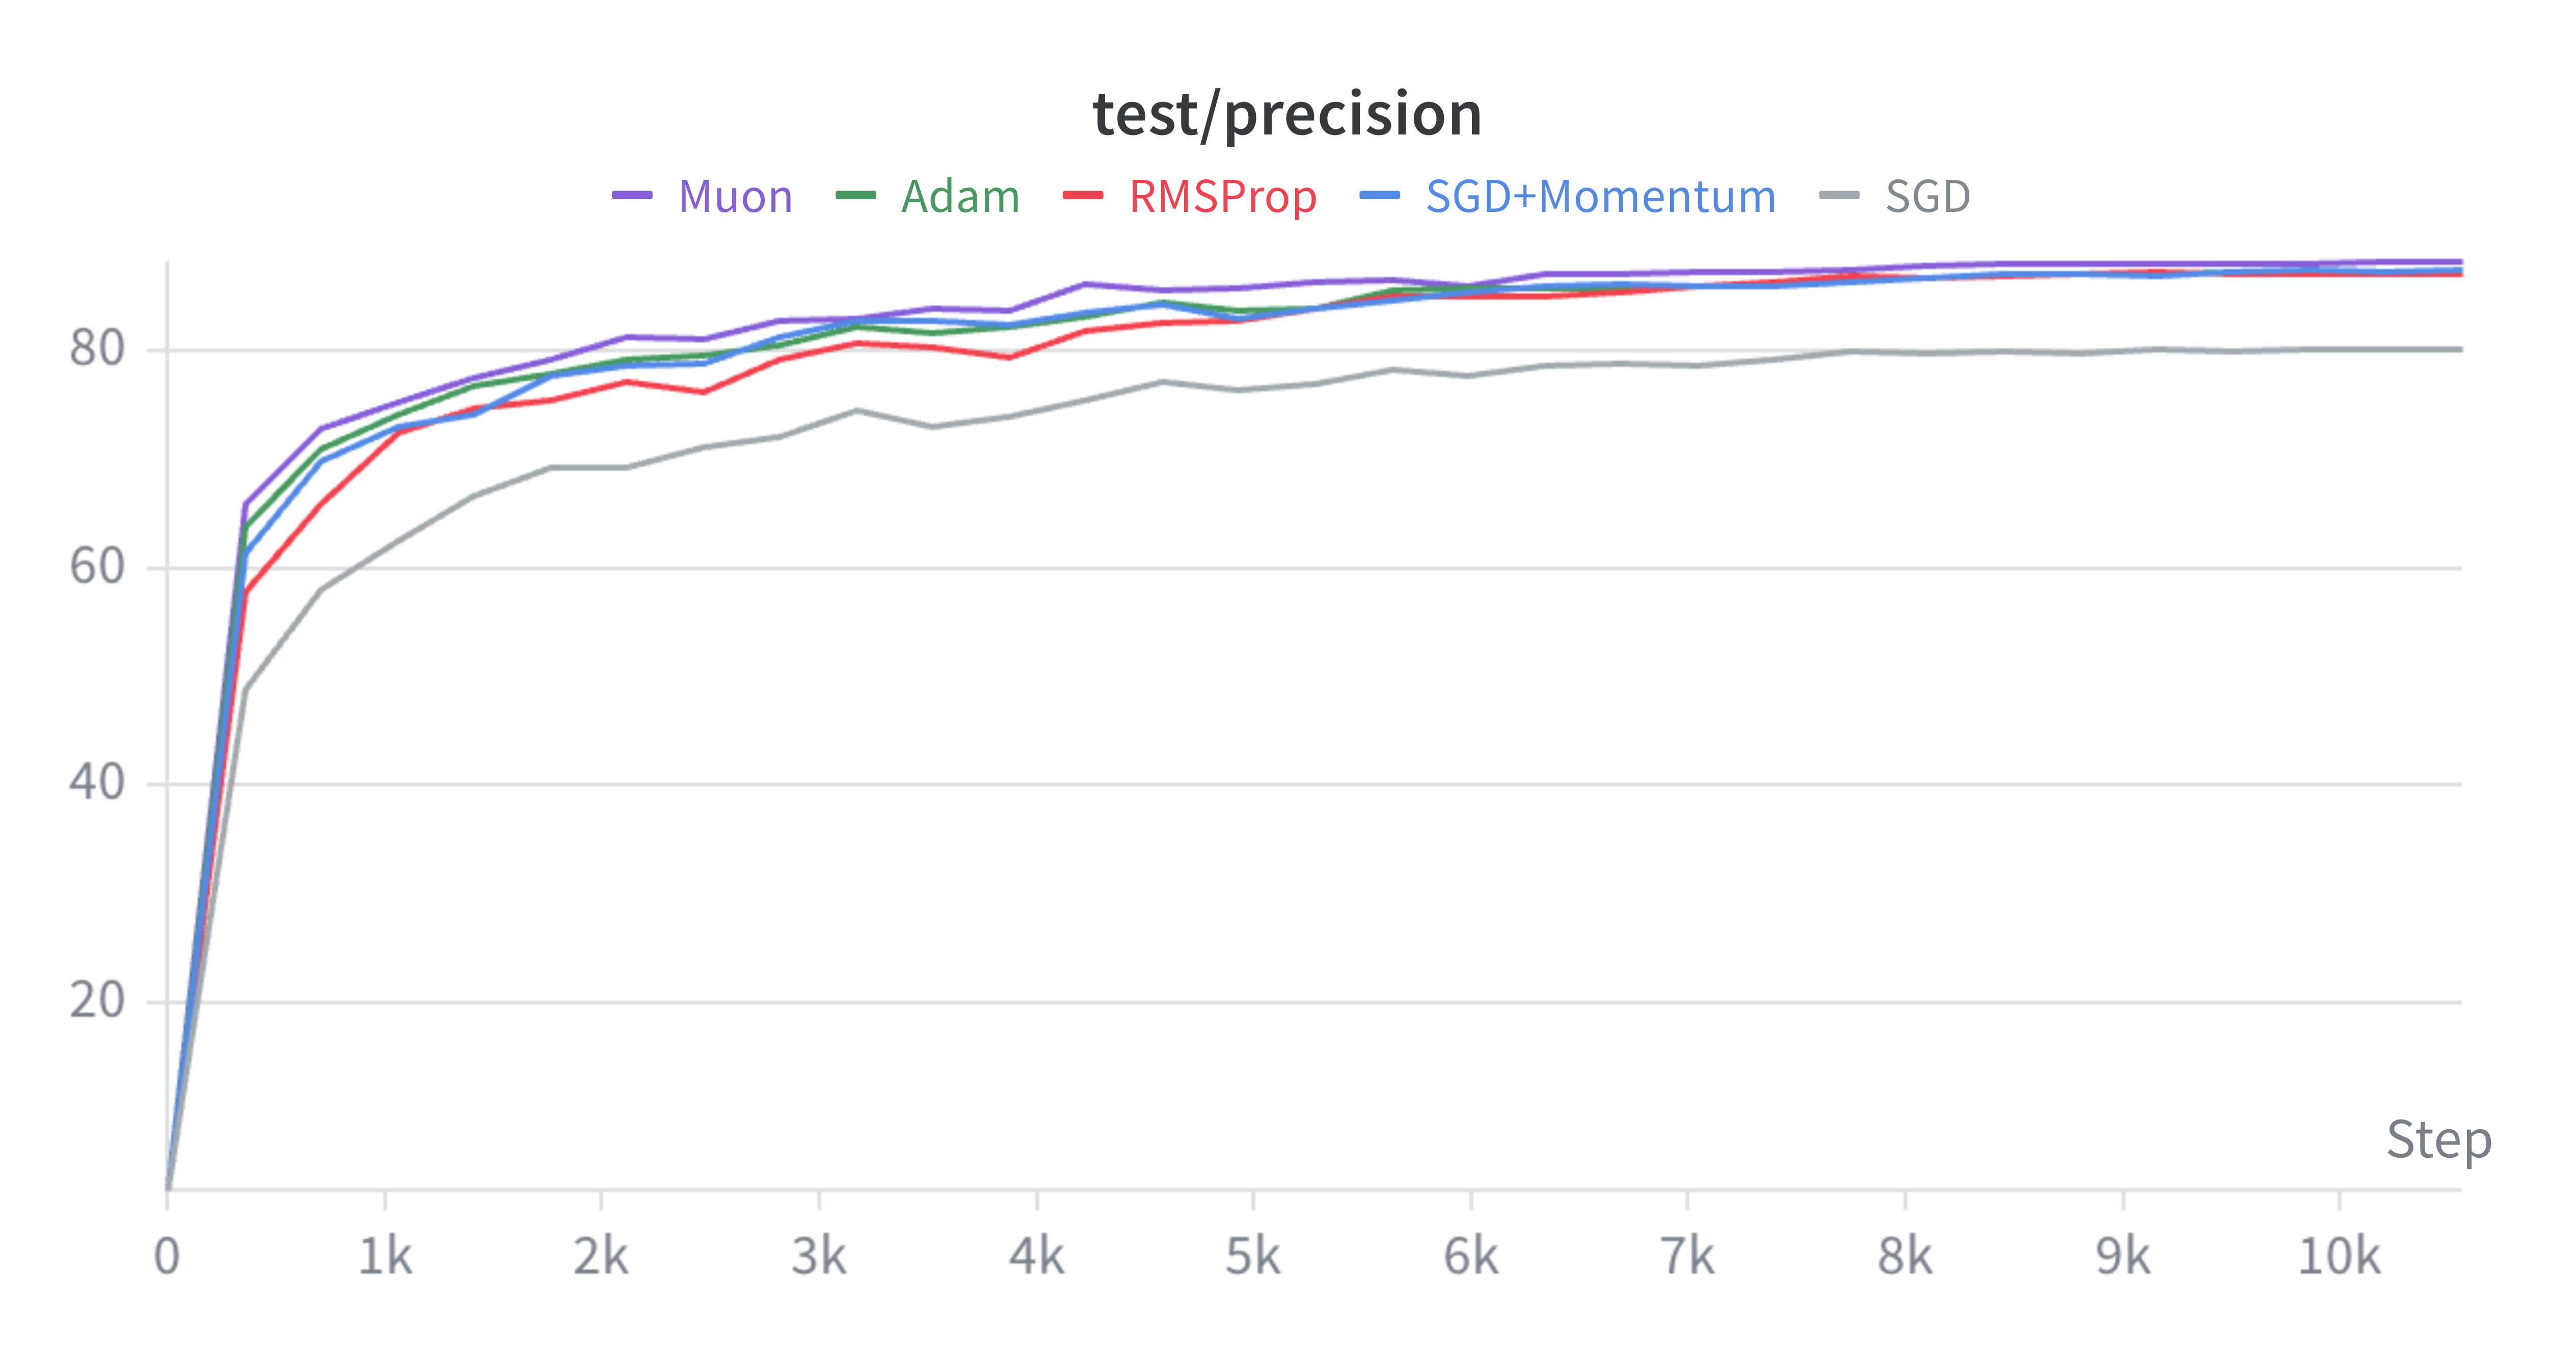
\includegraphics[width=\textwidth]{images/test-precision.png}
    \caption{Precision de test}
  \end{subfigure}

  \caption{Courbes d'accuracy pour les cinq optimiseurs (30 époques)}
  \label{fig:pre-curves}
\end{figure}

  \begin{table}[H]
    \centering
    \caption{Résumé des performances finales des cinq optimiseurs après 30 époques}
    \label{tab:optimizer-summary}
    \resizebox{\textwidth}{!}{%
    \begin{tabular}{lccccccc}
      \toprule
      Optimiseur & Train acc. (\%) & Val acc. (\%) & Val precision (\%) & Test acc. (\%) & Test precision (\%) & Gap génér. (\%) & Epochs val $
      \rightarrow$ 80\% \\
      \midrule
      SGD          & 80.90 & 81.04 & 80.97 & 80.31 & 80.22 & -0.04 & 22 \\
      SGD+Momentum & 91.34 & 88.10 & 88.04 & 87.53 & 87.52 & 3.36  & 8  \\
      RMSProp      & 91.31 & 88.00 & 87.97 & 87.34 & 87.32 & 3.31  & 12 \\
      Adam         & 91.84 & 87.80 & 87.73 & 87.34 & 87.35 & 4.10  & 8  \\
      Muon         & 92.96 & 89.00 & 88.91 & 88.25 & 88.22 & 3.96  & 6  \\
      \bottomrule
    \end{tabular}%
    }
  \end{table}

Les résultats montrent qu'Adam et SGD+Momentum sont les optimiseurs les plus
performants : 

Adam atteint la meilleure précision test finale (86.74\,\%),
tandis que SGD+Momentum obtient la meilleure précision test maximale (87.05\,\%),
un écart négligeable qui en fait deux choix équivalents dans notre configuration.
RMSProp se situe juste en dessous (85.84\,\%), suivi d'Muon (83.77\,\%), dont
le faible écart de généralisation ne compense pas une précision finale plus
modeste. SGD seul atteint 81.22\,\%, progressant correctement mais trop
lentement sur 30 epochs sans mécanisme d'adaptation.

Ces résultats illustrent un compromis entre vitesse de convergence et
généralisation : les méthodes adaptatives et à momentum atteignent de meilleures
précisions mais présentent un écart train-test plus marqué. Dans un budget de
30 epochs, Adam et SGD+Momentum s'imposent comme les choix les plus compétitifs.
\subsection{Sensibilité au taux d'apprentissage}


\subsection{Normes des gradients}

  

\begin{figure}[H]
    \centering
    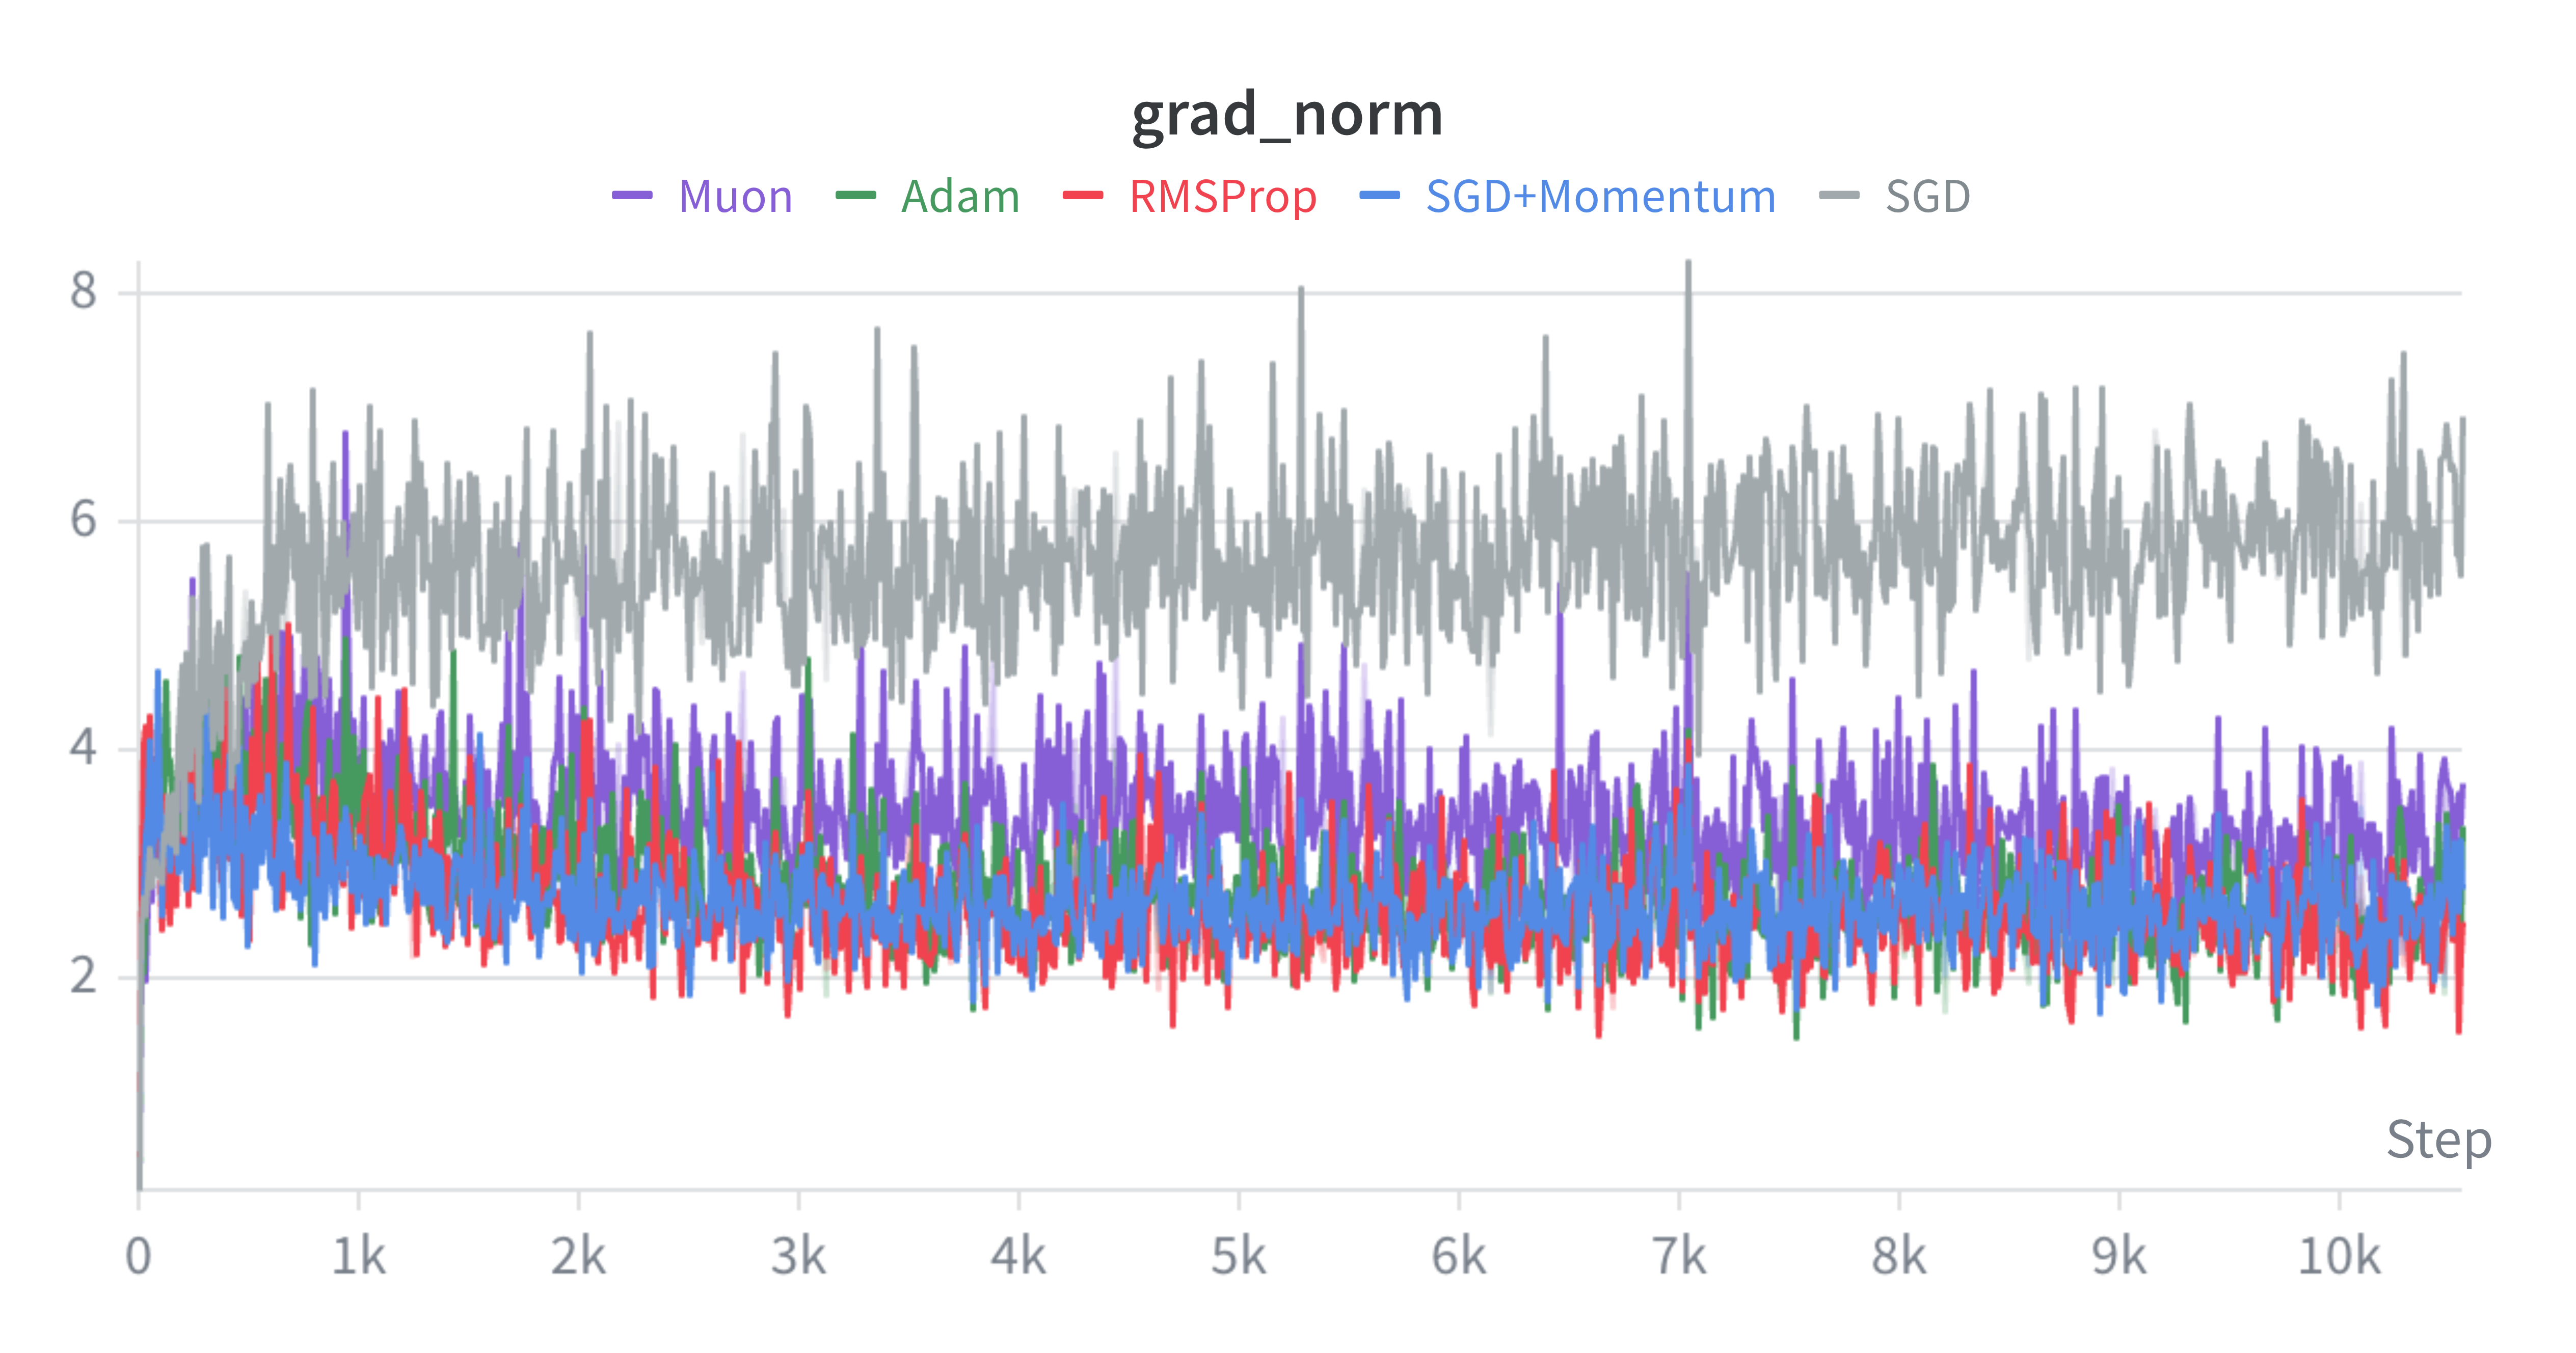
\includegraphics[width=\textwidth]{images/grad-norm.png}
    \caption{Normes des gradients}
    \label{fig:grad-norm}
\end{figure}

SGD+Momentum, Adam et RMSProp réduisent progressivement la norme des gradients, ce qui indique une stabilisation de l'entraînement et des mises à jour de plus en plus faibles. SGD+Momentum atteint les gradients les plus faibles en fin d'entraînement, suggérant une trajectoire plus régulière. À l'inverse, Muon conserve une norme plus élevée mais stable, ce qui traduit un comportement d'optimisation différent et peut expliquer sa performance finale moins compétitive.
% ==========================================================
\section{Discussion}

\subsection{Lien avec la non-convexité}

Les résultats illustrent les difficultés de l'optimisation non convexe : les
optimiseurs suivent des trajectoires différentes, visibles dans les courbes de
perte, les normes de gradient et les écarts de généralisation. SGD présente une
convergence plus lente et des gradients plus bruités, tandis qu'Adam, RMSProp
et SGD+Momentum stabilisent plus rapidement l'apprentissage grâce au momentum
et à l'adaptation du taux. Cependant, une convergence rapide s'accompagne d'un
écart train-test plus important, suggérant que la trajectoire influence non
seulement la vitesse, mais aussi le type de minimum atteint.

\subsection{Convergence et généralisation}

\begin{figure}[H]
    \centering
    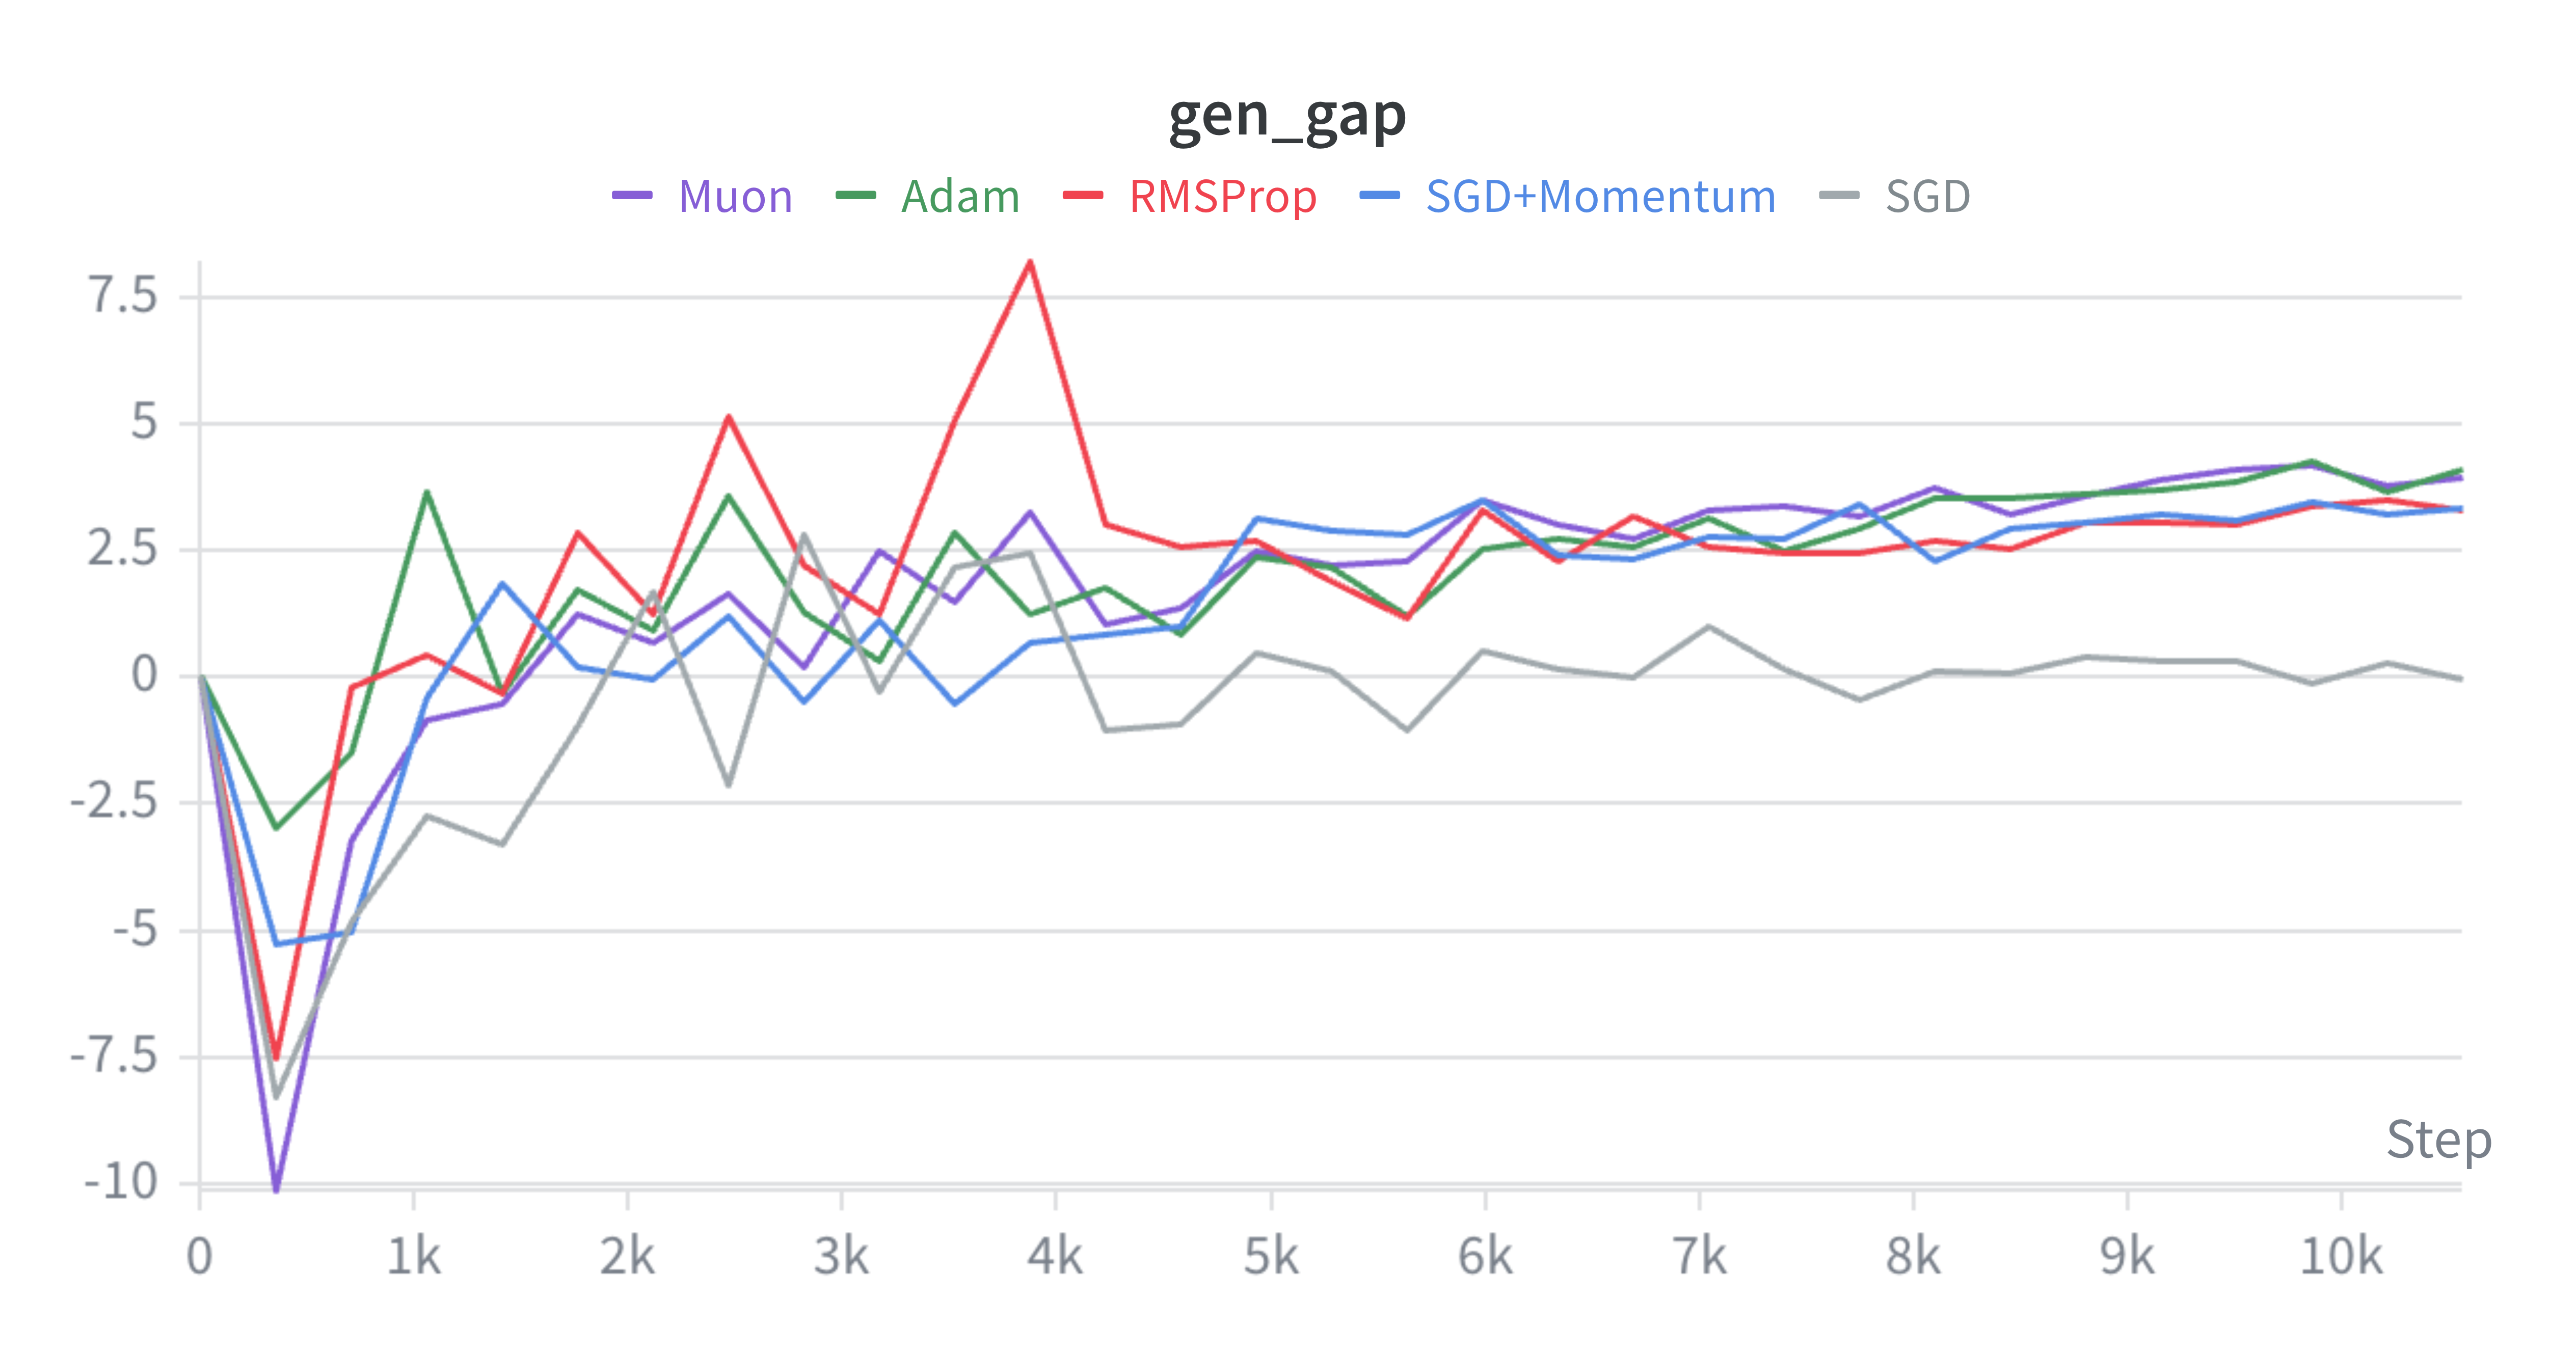
\includegraphics[width=\textwidth]{images/gen-gap.png}
    \caption{Écart de généralisation}
    \label{fig:gen-gap}
\end{figure}

La Figure~\ref{fig:gen-gap} compare l'écart de généralisation entre les
optimiseurs, défini comme la différence entre l'accuracy d'entraînement et
l'accuracy de test. Un écart plus élevé indique une tendance plus forte au
sur-apprentissage. Les résultats montrent qu'Adam obtient une très bonne
précision finale tout en gardant un écart plus faible que SGD+Momentum. Ainsi,
dans notre expérience, le paradoxe classique selon lequel Adam généralise moins
bien que SGD n'apparaît pas clairement ; on observe plutôt un compromis entre
vitesse de convergence, précision test et écart train-test.

\subsection{Limites de l'étude}

Le budget fixe de 30 epochs favorise les optimiseurs rapides ; un entraînement
plus long pourrait avantager SGD. Les résultats issus d'une seule exécution par
optimiseur ne permettent pas d'estimer la variance due à l'initialisation ou au
bruit stochastique. Enfin, la comparaison reste sensible aux hyperparamètres
choisis et à l'architecture utilisée ; les conclusions sont donc propres à ce
cadre expérimental.

% ==========================================================
\section{Conclusion}
\label{sec:conclusion}
% ==========================================================

Ce travail a mis en évidence que le choix de l'optimiseur influence fortement la
trajectoire d'apprentissage d'un CNN sur CIFAR-10. SGD seul converge de manière
stable mais reste nettement plus lent, tandis que SGD avec momentum, Adam,
RMSProp et Muon atteignent plus rapidement de meilleures performances. Les
résultats montrent aussi qu'une convergence rapide ne suffit pas à juger un
optimiseur : il faut également tenir compte de la précision finale, de la norme
des gradients et de l'écart de généralisation.

Dans notre cadre expérimental, les optimiseurs avec momentum ou adaptation du
taux d'apprentissage offrent le meilleur compromis entre vitesse et performance.
Les écarts observés restent toutefois dépendants du nombre limité d'époques, des
hyperparamètres choisis et de l'architecture utilisée.

\newpage
% ==========================================================
\begin{thebibliography}{99}

\bibitem{krizhevsky2009cifar}
Krizhevsky, A. (2009).
\textit{Learning Multiple Layers of Features from Tiny Images}.
Technical Report, University of Toronto.

\bibitem{he2016resnet}
He, K., Zhang, X., Ren, S., \& Sun, J. (2016).
\textit{Deep Residual Learning for Image Recognition}.
IEEE/CVF Conference on Computer Vision and Pattern Recognition (CVPR), 770--778.

\bibitem{simonyan2014vgg}
Simonyan, K., \& Zisserman, A. (2014).
\textit{Very Deep Convolutional Networks for Large-Scale Image Recognition}.
International Conference on Learning Representations (ICLR).

\bibitem{huang2017densenet}
Huang, G., Liu, Z., Van der Maaten, L., \& Weinberger, K. Q. (2017).
\textit{Densely Connected Convolutional Networks}.
IEEE/CVF Conference on Computer Vision and Pattern Recognition (CVPR), 4700--4708.

\bibitem{kingma2014adam}
Kingma, D. P., \& Ba, J. (2015).
\textit{Adam: A Method for Stochastic Optimization}.
International Conference on Learning Representations (ICLR).

\bibitem{jordan2024muon}
Jordan, K., Jin, Y., Boza, V., Jiacheng, Y., Cesista, F., Newhouse, L., \& Bernstein, J. (2024).
\textit{Muon: An optimizer for hidden layers in neural networks}.


\bibitem{hinton2012rmsprop}
Tieleman, T., \& Hinton, G. (2012).
\textit{Lecture 6.5 — RMSProp: Divide the gradient by a running average of its recent magnitude}.
COURSERA: Neural Networks for Machine Learning.

\bibitem{wilson2017marginal}
Wilson, A. C., Roelofs, R., Stern, M., Srebro, N., \& Recht, B. (2017).
\textit{The Marginal Value of Momentum for Small Learning Rate SGD}.
International Conference on Learning Representations (ICLR).


\end{thebibliography}

\end{document}
